\documentclass[1p]{elsarticle_modified}
%\bibliographystyle{elsarticle-num}

%\usepackage[colorlinks]{hyperref}
%\usepackage{abbrmath_seonhwa} %\Abb, \Ascr, \Acal ,\Abf, \Afrak
\usepackage{amsfonts}
\usepackage{amssymb}
\usepackage{amsmath}
\usepackage{amsthm}
\usepackage{scalefnt}
\usepackage{amsbsy}
\usepackage{kotex}
\usepackage{caption}
\usepackage{subfig}
\usepackage{color}
\usepackage{graphicx}
\usepackage{xcolor} %% white, black, red, green, blue, cyan, magenta, yellow
\usepackage{float}
\usepackage{setspace}
\usepackage{hyperref}

\usepackage{tikz}
\usetikzlibrary{arrows}

\usepackage{multirow}
\usepackage{array} % fixed length table
\usepackage{hhline}

%%%%%%%%%%%%%%%%%%%%%
\makeatletter
\renewcommand*\env@matrix[1][\arraystretch]{%
	\edef\arraystretch{#1}%
	\hskip -\arraycolsep
	\let\@ifnextchar\new@ifnextchar
	\array{*\c@MaxMatrixCols c}}
\makeatother %https://tex.stackexchange.com/questions/14071/how-can-i-increase-the-line-spacing-in-a-matrix
%%%%%%%%%%%%%%%

\usepackage[normalem]{ulem}

\newcommand{\msout}[1]{\ifmmode\text{\sout{\ensuremath{#1}}}\else\sout{#1}\fi}
%SOURCE: \msout is \stkout macro in https://tex.stackexchange.com/questions/20609/strikeout-in-math-mode

\newcommand{\cancel}[1]{
	\ifmmode
	{\color{red}\msout{#1}}
	\else
	{\color{red}\sout{#1}}
	\fi
}

\newcommand{\add}[1]{
	{\color{blue}\uwave{#1}}
}

\newcommand{\replace}[2]{
	\ifmmode
	{\color{red}\msout{#1}}{\color{blue}\uwave{#2}}
	\else
	{\color{red}\sout{#1}}{\color{blue}\uwave{#2}}
	\fi
}

\newcommand{\Sol}{\mathcal{S}} %segment
\newcommand{\D}{D} %diagram
\newcommand{\A}{\mathcal{A}} %arc


%%%%%%%%%%%%%%%%%%%%%%%%%%%%%5 test

\def\sl{\operatorname{\textup{SL}}(2,\Cbb)}
\def\psl{\operatorname{\textup{PSL}}(2,\Cbb)}
\def\quan{\mkern 1mu \triangleright \mkern 1mu}

\theoremstyle{definition}
\newtheorem{thm}{Theorem}[section]
\newtheorem{prop}[thm]{Proposition}
\newtheorem{lem}[thm]{Lemma}
\newtheorem{ques}[thm]{Question}
\newtheorem{cor}[thm]{Corollary}
\newtheorem{defn}[thm]{Definition}
\newtheorem{exam}[thm]{Example}
\newtheorem{rmk}[thm]{Remark}
\newtheorem{alg}[thm]{Algorithm}

\newcommand{\I}{\sqrt{-1}}
\begin{document}

%\begin{frontmatter}
%
%\title{Boundary parabolic representations of knots up to 8 crossings}
%
%%% Group authors per affiliation:
%\author{Yunhi Cho} 
%\address{Department of Mathematics, University of Seoul, Seoul, Korea}
%\ead{yhcho@uos.ac.kr}
%
%
%\author{Seonhwa Kim} %\fnref{s_kim}}
%\address{Center for Geometry and Physics, Institute for Basic Science, Pohang, 37673, Korea}
%\ead{ryeona17@ibs.re.kr}
%
%\author{Hyuk Kim}
%\address{Department of Mathematical Sciences, Seoul National University, Seoul 08826, Korea}
%\ead{hyukkim@snu.ac.kr}
%
%\author{Seokbeom Yoon}
%\address{Department of Mathematical Sciences, Seoul National University, Seoul, 08826,  Korea}
%\ead{sbyoon15@snu.ac.kr}
%
%\begin{abstract}
%We find all boundary parabolic representation of knots up to 8 crossings.
%
%\end{abstract}
%\begin{keyword}
%    \MSC[2010] 57M25 
%\end{keyword}
%
%\end{frontmatter}

%\linenumbers
%\tableofcontents
%
\newcommand\colored[1]{\textcolor{white}{\rule[-0.35ex]{0.8em}{1.4ex}}\kern-0.8em\color{red} #1}%
%\newcommand\colored[1]{\textcolor{white}{ #1}\kern-2.17ex	\textcolor{white}{ #1}\kern-1.81ex	\textcolor{white}{ #1}\kern-2.15ex\color{red}#1	}

{\Large $\underline{12n_{0887}~(K12n_{0887})}$}

\setlength{\tabcolsep}{10pt}
\renewcommand{\arraystretch}{1.6}
\vspace{1cm}\begin{tabular}{m{100pt}>{\centering\arraybackslash}m{274pt}}
\multirow{5}{120pt}{
	\centering
	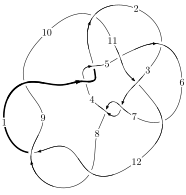
\includegraphics[width=112pt]{../../../GIT/diagram.site/Diagrams/png/2976_12n_0887.png}\\
\ \ \ A knot diagram\footnotemark}&
\allowdisplaybreaks
\textbf{Linearized knot diagam} \\
\cline{2-2}
 &
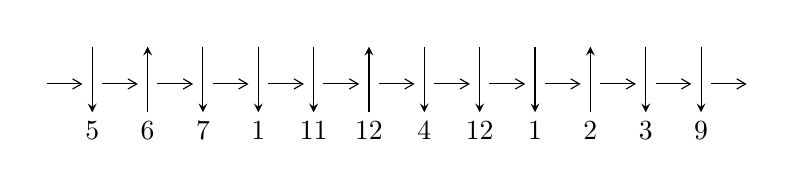
\begin{tikzpicture}[x=20pt, y=17pt]
	% nodes
	\node (C0) at (0, 0) {};
	\node (C1) at (1, 0) {};
	\node (C1U) at (1, +1) {};
	\node (C1D) at (1, -1) {5};

	\node (C2) at (2, 0) {};
	\node (C2U) at (2, +1) {};
	\node (C2D) at (2, -1) {6};

	\node (C3) at (3, 0) {};
	\node (C3U) at (3, +1) {};
	\node (C3D) at (3, -1) {7};

	\node (C4) at (4, 0) {};
	\node (C4U) at (4, +1) {};
	\node (C4D) at (4, -1) {1};

	\node (C5) at (5, 0) {};
	\node (C5U) at (5, +1) {};
	\node (C5D) at (5, -1) {11};

	\node (C6) at (6, 0) {};
	\node (C6U) at (6, +1) {};
	\node (C6D) at (6, -1) {12};

	\node (C7) at (7, 0) {};
	\node (C7U) at (7, +1) {};
	\node (C7D) at (7, -1) {4};

	\node (C8) at (8, 0) {};
	\node (C8U) at (8, +1) {};
	\node (C8D) at (8, -1) {12};

	\node (C9) at (9, 0) {};
	\node (C9U) at (9, +1) {};
	\node (C9D) at (9, -1) {1};

	\node (C10) at (10, 0) {};
	\node (C10U) at (10, +1) {};
	\node (C10D) at (10, -1) {2};

	\node (C11) at (11, 0) {};
	\node (C11U) at (11, +1) {};
	\node (C11D) at (11, -1) {3};

	\node (C12) at (12, 0) {};
	\node (C12U) at (12, +1) {};
	\node (C12D) at (12, -1) {9};
	\node (C13) at (13, 0) {};

	% arrows
	\draw[->,>={angle 60}]
	(C0) edge (C1) (C1) edge (C2) (C2) edge (C3) (C3) edge (C4) (C4) edge (C5) (C5) edge (C6) (C6) edge (C7) (C7) edge (C8) (C8) edge (C9) (C9) edge (C10) (C10) edge (C11) (C11) edge (C12) (C12) edge (C13) ;	\draw[->,>=stealth]
	(C1U) edge (C1D) (C2D) edge (C2U) (C3U) edge (C3D) (C4U) edge (C4D) (C5U) edge (C5D) (C6D) edge (C6U) (C7U) edge (C7D) (C8U) edge (C8D) (C9U) edge (C9D) (C10D) edge (C10U) (C11U) edge (C11D) (C12U) edge (C12D) ;
	\end{tikzpicture} \\
\hhline{~~} \\& 
\textbf{Solving Sequence} \\ \cline{2-2} 
 &
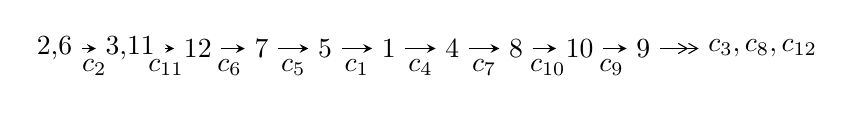
\begin{tikzpicture}[x=23pt, y=7pt]
	% node
	\node (A0) at (-1/8, 0) {2,6};
	\node (A1) at (17/16, 0) {3,11};
	\node (A2) at (17/8, 0) {12};
	\node (A3) at (25/8, 0) {7};
	\node (A4) at (33/8, 0) {5};
	\node (A5) at (41/8, 0) {1};
	\node (A6) at (49/8, 0) {4};
	\node (A7) at (57/8, 0) {8};
	\node (A8) at (65/8, 0) {10};
	\node (A9) at (73/8, 0) {9};
	\node (C1) at (1/2, -1) {$c_{2}$};
	\node (C2) at (13/8, -1) {$c_{11}$};
	\node (C3) at (21/8, -1) {$c_{6}$};
	\node (C4) at (29/8, -1) {$c_{5}$};
	\node (C5) at (37/8, -1) {$c_{1}$};
	\node (C6) at (45/8, -1) {$c_{4}$};
	\node (C7) at (53/8, -1) {$c_{7}$};
	\node (C8) at (61/8, -1) {$c_{10}$};
	\node (C9) at (69/8, -1) {$c_{9}$};
	\node (A10) at (11, 0) {$c_{3},c_{8},c_{12}$};

	% edge
	\draw[->,>=stealth]	
	(A0) edge (A1) (A1) edge (A2) (A2) edge (A3) (A3) edge (A4) (A4) edge (A5) (A5) edge (A6) (A6) edge (A7) (A7) edge (A8) (A8) edge (A9) ;
	\draw[->>,>={angle 60}]	
	(A9) edge (A10);
\end{tikzpicture} \\ 

\end{tabular} \\

\footnotetext{
The image of knot diagram is generated by the software ``\textbf{Draw programme}" developed by Andrew Bartholomew(\url{http://www.layer8.co.uk/maths/draw/index.htm\#Running-draw}), where we modified some parts for our purpose(\url{https://github.com/CATsTAILs/LinksPainter}).
}\phantom \\ \newline 
\centering \textbf{Ideals for irreducible components\footnotemark of $X_{\text{par}}$} 
 
\begin{align*}
I^u_{1}&=\langle 
b+u,\;- u^4-2 u^3-2 u^2+a-2,\;u^5+3 u^4+4 u^3+2 u^2+2 u+1\rangle \\
I^u_{2}&=\langle 
b+u,\;-270959 u^{13}+772689 u^{12}+\cdots+300046 a-41334,\\
\phantom{I^u_{2}}&\phantom{= \langle  }u^{14}-2 u^{13}- u^{12}+2 u^{11}+10 u^{10}-9 u^9-29 u^8+46 u^7+16 u^6-61 u^5+18 u^4+22 u^3-14 u^2+3 u-1\rangle \\
I^u_{3}&=\langle 
-135792 u^{13}+108799 u^{12}+\cdots+300046 b+457605,\\
\phantom{I^u_{3}}&\phantom{= \langle  }-230771 u^{13}+274896 u^{12}+\cdots+300046 a-29087,\\
\phantom{I^u_{3}}&\phantom{= \langle  }u^{14}-2 u^{13}- u^{12}+2 u^{11}+10 u^{10}-9 u^9-29 u^8+46 u^7+16 u^6-61 u^5+18 u^4+22 u^3-14 u^2+3 u-1\rangle \\
I^u_{4}&=\langle 
-104218005 u^{13}+702274247 u^{12}+\cdots+190982362 b+773333180,\\
\phantom{I^u_{4}}&\phantom{= \langle  }544231529 u^{13}-3353087149 u^{12}+\cdots+763929448 a-3082001714,\;u^{14}-7 u^{13}+\cdots-8 u+4\rangle \\
I^u_{5}&=\langle 
-180047861 u^{13}+1175460277 u^{12}+\cdots+381964724 b+1337790626,\\
\phantom{I^u_{5}}&\phantom{= \langle  }158399813 u^{13}-1046466799 u^{12}+\cdots+381964724 a-2606371288,\;u^{14}-7 u^{13}+\cdots-8 u+4\rangle \\
I^u_{6}&=\langle 
-103563766675 u^{13}-565696363294 u^{12}+\cdots+912579422726 b+472806896800,\\
\phantom{I^u_{6}}&\phantom{= \langle  }218496302654 u^{13}+1210683237470 u^{12}+\cdots+912579422726 a-6915383452949,\\
\phantom{I^u_{6}}&\phantom{= \langle  }u^{14}+6 u^{13}+\cdots-22 u+4\rangle \\
I^u_{7}&=\langle 
b+u,\;u^2+a- u+2,\;u^3-2 u^2+3 u-1\rangle \\
I^u_{8}&=\langle 
b,\;a+u+1,\;u^2+u-1\rangle \\
I^u_{9}&=\langle 
b,\;a^2- a-1,\;u-1\rangle \\
I^u_{10}&=\langle 
b+u,\;a+1,\;u^2+u-1\rangle \\
\\
I^v_{1}&=\langle 
a,\;b+1,\;v^2- v-1\rangle \\
I^v_{2}&=\langle 
a,\;b- v-1,\;v^2+v-1\rangle \\
\end{align*}
\raggedright * 12 irreducible components of $\dim_{\mathbb{C}}=0$, with total 88 representations.\\
\footnotetext{All coefficients of polynomials are rational numbers. But the coefficients are sometimes approximated in decimal forms when there is not enough margin.}
\newpage
\renewcommand{\arraystretch}{1}
\centering \section*{I. $I^u_{1}= \langle b+u,\;- u^4-2 u^3-2 u^2+a-2,\;u^5+3 u^4+4 u^3+2 u^2+2 u+1 \rangle$}
\flushleft \textbf{(i) Arc colorings}\\
\begin{tabular}{m{7pt} m{180pt} m{7pt} m{180pt} }
\flushright $a_{2}=$&$\begin{pmatrix}1\\0\end{pmatrix}$ \\
\flushright $a_{6}=$&$\begin{pmatrix}0\\u\end{pmatrix}$ \\
\flushright $a_{3}=$&$\begin{pmatrix}1\\- u^2\end{pmatrix}$ \\
\flushright $a_{11}=$&$\begin{pmatrix}u^4+2 u^3+2 u^2+2\\- u\end{pmatrix}$ \\
\flushright $a_{12}=$&$\begin{pmatrix}1\\u^4+2 u^3+u^2+1\end{pmatrix}$ \\
\flushright $a_{7}=$&$\begin{pmatrix}u\\- u^4-3 u^3-2 u^2-1\end{pmatrix}$ \\
\flushright $a_{5}=$&$\begin{pmatrix}-2 u^4-5 u^3-5 u^2- u-3\\- u^4-2 u^3-2 u^2-1\end{pmatrix}$ \\
\flushright $a_{1}=$&$\begin{pmatrix}-2 u^4-5 u^3-6 u^2- u-3\\- u^4-3 u^3-3 u^2- u-2\end{pmatrix}$ \\
\flushright $a_{4}=$&$\begin{pmatrix}u^4+2 u^3+2 u^2+u+2\\u^2+1\end{pmatrix}$ \\
\flushright $a_{8}=$&$\begin{pmatrix}u^4+3 u^3+3 u^2+u+2\\u^4+u^3+u^2+u+1\end{pmatrix}$ \\
\flushright $a_{10}=$&$\begin{pmatrix}u^4+2 u^3+2 u^2+u+2\\- u\end{pmatrix}$ \\
\flushright $a_{9}=$&$\begin{pmatrix}-2 u^4-5 u^3-5 u^2- u-3\\- u^4-2 u^3-3 u^2- u-2\end{pmatrix}$\\&\end{tabular}
\flushleft \textbf{(ii) Obstruction class $= -1$}\\~\\
\flushleft \textbf{(iii) Cusp Shapes $= -5 u^4-10 u^3-10 u^2+5 u-14$}\\~\\
\newpage\renewcommand{\arraystretch}{1}
\flushleft \textbf{(iv) u-Polynomials at the component}\newline \\
\begin{tabular}{m{50pt}|m{274pt}}
Crossings & \hspace{64pt}u-Polynomials at each crossing \\
\hline $$\begin{aligned}c_{1},c_{3},c_{4}\\c_{5},c_{7},c_{8}\\c_{9},c_{11},c_{12}\end{aligned}$$&$\begin{aligned}
&u^5+2 u^4-4 u^2-3 u-1
\end{aligned}$\\
\hline $$\begin{aligned}c_{2},c_{6},c_{10}\end{aligned}$$&$\begin{aligned}
&u^5-3 u^4+4 u^3-2 u^2+2 u-1
\end{aligned}$\\
\hline
\end{tabular}\\~\\
\newpage\renewcommand{\arraystretch}{1}
\flushleft \textbf{(v) Riley Polynomials at the component}\newline \\
\begin{tabular}{m{50pt}|m{274pt}}
Crossings & \hspace{64pt}Riley Polynomials at each crossing \\
\hline $$\begin{aligned}c_{1},c_{3},c_{4}\\c_{5},c_{7},c_{8}\\c_{9},c_{11},c_{12}\end{aligned}$$&$\begin{aligned}
&y^5-4 y^4+10 y^3-12 y^2+y-1
\end{aligned}$\\
\hline $$\begin{aligned}c_{2},c_{6},c_{10}\end{aligned}$$&$\begin{aligned}
&y^5- y^4+8 y^3+6 y^2-1
\end{aligned}$\\
\hline
\end{tabular}\\~\\
\newpage\flushleft \textbf{(vi) Complex Volumes and Cusp Shapes}
$$\begin{array}{c|c|c}  
\text{Solutions to }I^u_{1}& \I (\text{vol} + \sqrt{-1}CS) & \text{Cusp shape}\\
 \hline 
\begin{aligned}
u &= \phantom{-}0.179794 + 0.731571 I \\
a &= \phantom{-}0.612209 - 0.379621 I \\
b &= -0.179794 - 0.731571 I\end{aligned}
 & -0.867863 - 1.011200 I & -6.16207 + 5.55596 I \\ \hline\begin{aligned}
u &= \phantom{-}0.179794 - 0.731571 I \\
a &= \phantom{-}0.612209 + 0.379621 I \\
b &= -0.179794 + 0.731571 I\end{aligned}
 & -0.867863 + 1.011200 I & -6.16207 - 5.55596 I \\ \hline\begin{aligned}
u &= -0.583195\phantom{ +0.000000I} \\
a &= \phantom{-}2.39920\phantom{ +0.000000I} \\
b &= \phantom{-}0.583195\phantom{ +0.000000I}\end{aligned}
 & -12.9336\phantom{ +0.000000I} & -18.9120\phantom{ +0.000000I} \\ \hline\begin{aligned}
u &= -1.38820 + 1.04608 I \\
a &= -0.311811 - 0.840240 I \\
b &= \phantom{-}1.38820 - 1.04608 I\end{aligned}
 & -0.8900 - 17.3034 I & -9.38193 + 9.43159 I \\ \hline\begin{aligned}
u &= -1.38820 - 1.04608 I \\
a &= -0.311811 + 0.840240 I \\
b &= \phantom{-}1.38820 + 1.04608 I\end{aligned}
 & -0.8900 + 17.3034 I & -9.38193 - 9.43159 I\\
 \hline 
 \end{array}$$\newpage\newpage\renewcommand{\arraystretch}{1}
\centering \section*{II. $I^u_{2}= \langle b+u,\;-2.71\times10^{5} u^{13}+7.73\times10^{5} u^{12}+\cdots+3.00\times10^{5} a-4.13\times10^{4},\;u^{14}-2 u^{13}+\cdots+3 u-1 \rangle$}
\flushleft \textbf{(i) Arc colorings}\\
\begin{tabular}{m{7pt} m{180pt} m{7pt} m{180pt} }
\flushright $a_{2}=$&$\begin{pmatrix}1\\0\end{pmatrix}$ \\
\flushright $a_{6}=$&$\begin{pmatrix}0\\u\end{pmatrix}$ \\
\flushright $a_{3}=$&$\begin{pmatrix}1\\- u^2\end{pmatrix}$ \\
\flushright $a_{11}=$&$\begin{pmatrix}0.903058 u^{13}-2.57524 u^{12}+\cdots-24.1076 u+0.137759\\- u\end{pmatrix}$ \\
\flushright $a_{12}=$&$\begin{pmatrix}1.52512 u^{13}-3.50280 u^{12}+\cdots-26.3180 u+0.906878\\-0.0795245 u^{13}+0.200289 u^{12}+\cdots-0.672414 u-0.316548\end{pmatrix}$ \\
\flushright $a_{7}=$&$\begin{pmatrix}2.15993 u^{13}-4.52017 u^{12}+\cdots-23.6907 u-9.18261\\0.882721 u^{13}-0.910147 u^{12}+\cdots-2.84412 u+0.797954\end{pmatrix}$ \\
\flushright $a_{5}=$&$\begin{pmatrix}3.24733 u^{13}-5.66143 u^{12}+\cdots-27.2367 u-6.98262\\0.622058 u^{13}-0.927568 u^{12}+\cdots-2.21041 u+0.769119\end{pmatrix}$ \\
\flushright $a_{1}=$&$\begin{pmatrix}2.48254 u^{13}-4.44656 u^{12}+\cdots-20.0427 u+1.25212\\-1.00470 u^{13}+1.07172 u^{12}+\cdots+2.53232 u-1.63459\end{pmatrix}$ \\
\flushright $a_{4}=$&$\begin{pmatrix}4.54266 u^{13}-6.82224 u^{12}+\cdots-22.7975 u-5.41276\\-1.44675 u^{13}+2.26522 u^{12}+\cdots+0.459690 u-0.830456\end{pmatrix}$ \\
\flushright $a_{8}=$&$\begin{pmatrix}0.842261 u^{13}-0.940929 u^{12}+\cdots-12.2541 u-1.81451\\0.403411 u^{13}-0.923072 u^{12}+\cdots-1.22177 u+0.811476\end{pmatrix}$ \\
\flushright $a_{10}=$&$\begin{pmatrix}0.903058 u^{13}-2.57524 u^{12}+\cdots-23.1076 u+0.137759\\- u\end{pmatrix}$ \\
\flushright $a_{9}=$&$\begin{pmatrix}1.43263 u^{13}-2.87432 u^{12}+\cdots-11.5747 u+2.51098\\-1.18195 u^{13}+2.15844 u^{12}+\cdots+0.00298621 u-0.593296\end{pmatrix}$\\&\end{tabular}
\flushleft \textbf{(ii) Obstruction class $= -1$}\\~\\
\flushleft \textbf{(iii) Cusp Shapes $= \frac{5034313}{300046} u^{13}-\frac{7498729}{300046} u^{12}+\cdots-\frac{19035683}{300046} u-\frac{5404048}{150023}$}\\~\\
\newpage\renewcommand{\arraystretch}{1}
\flushleft \textbf{(iv) u-Polynomials at the component}\newline \\
\begin{tabular}{m{50pt}|m{274pt}}
Crossings & \hspace{64pt}u-Polynomials at each crossing \\
\hline $$\begin{aligned}c_{1},c_{4},c_{11}\end{aligned}$$&$\begin{aligned}
&u^{14}-3 u^{13}+\cdots+4 u-1
\end{aligned}$\\
\hline $$\begin{aligned}c_{2},c_{10}\end{aligned}$$&$\begin{aligned}
&u^{14}+2 u^{13}+\cdots-3 u-1
\end{aligned}$\\
\hline $$\begin{aligned}c_{3},c_{7},c_{8}\\c_{9},c_{12}\end{aligned}$$&$\begin{aligned}
&u^{14}-2 u^{13}+\cdots+3 u+1
\end{aligned}$\\
\hline $$\begin{aligned}c_{5}\end{aligned}$$&$\begin{aligned}
&u^{14}+11 u^{13}+\cdots+32 u+16
\end{aligned}$\\
\hline $$\begin{aligned}c_{6}\end{aligned}$$&$\begin{aligned}
&u^{14}+7 u^{13}+\cdots+8 u+4
\end{aligned}$\\
\hline
\end{tabular}\\~\\
\newpage\renewcommand{\arraystretch}{1}
\flushleft \textbf{(v) Riley Polynomials at the component}\newline \\
\begin{tabular}{m{50pt}|m{274pt}}
Crossings & \hspace{64pt}Riley Polynomials at each crossing \\
\hline $$\begin{aligned}c_{1},c_{4},c_{11}\end{aligned}$$&$\begin{aligned}
&y^{14}-5 y^{13}+\cdots-12 y+1
\end{aligned}$\\
\hline $$\begin{aligned}c_{2},c_{10}\end{aligned}$$&$\begin{aligned}
&y^{14}-6 y^{13}+\cdots+19 y+1
\end{aligned}$\\
\hline $$\begin{aligned}c_{3},c_{7},c_{8}\\c_{9},c_{12}\end{aligned}$$&$\begin{aligned}
&y^{14}-6 y^{13}+\cdots-29 y+1
\end{aligned}$\\
\hline $$\begin{aligned}c_{5}\end{aligned}$$&$\begin{aligned}
&y^{14}-3 y^{13}+\cdots-1952 y+256
\end{aligned}$\\
\hline $$\begin{aligned}c_{6}\end{aligned}$$&$\begin{aligned}
&y^{14}-3 y^{13}+\cdots-200 y+16
\end{aligned}$\\
\hline
\end{tabular}\\~\\
\newpage\flushleft \textbf{(vi) Complex Volumes and Cusp Shapes}
$$\begin{array}{c|c|c}  
\text{Solutions to }I^u_{2}& \I (\text{vol} + \sqrt{-1}CS) & \text{Cusp shape}\\
 \hline 
\begin{aligned}
u &= -1.047510 + 0.114828 I \\
a &= -0.341221 - 0.956988 I \\
b &= \phantom{-}1.047510 - 0.114828 I\end{aligned}
 & \phantom{-}4.40804 - 3.15243 I & -3.06554 + 3.15957 I \\ \hline\begin{aligned}
u &= -1.047510 - 0.114828 I \\
a &= -0.341221 + 0.956988 I \\
b &= \phantom{-}1.047510 + 0.114828 I\end{aligned}
 & \phantom{-}4.40804 + 3.15243 I & -3.06554 - 3.15957 I \\ \hline\begin{aligned}
u &= -1.12842\phantom{ +0.000000I} \\
a &= \phantom{-}0.452479\phantom{ +0.000000I} \\
b &= \phantom{-}1.12842\phantom{ +0.000000I}\end{aligned}
 & -9.22310\phantom{ +0.000000I} & -8.50330\phantom{ +0.000000I} \\ \hline\begin{aligned}
u &= \phantom{-}0.798926 + 0.304657 I \\
a &= \phantom{-}0.99674 + 1.31288 I \\
b &= -0.798926 - 0.304657 I\end{aligned}
 & \phantom{-}1.89333 + 9.70124 I & -6.29823 - 7.45288 I \\ \hline\begin{aligned}
u &= \phantom{-}0.798926 - 0.304657 I \\
a &= \phantom{-}0.99674 - 1.31288 I \\
b &= -0.798926 + 0.304657 I\end{aligned}
 & \phantom{-}1.89333 - 9.70124 I & -6.29823 + 7.45288 I \\ \hline\begin{aligned}
u &= \phantom{-}0.814809\phantom{ +0.000000I} \\
a &= -0.638076\phantom{ +0.000000I} \\
b &= -0.814809\phantom{ +0.000000I}\end{aligned}
 & -2.25467\phantom{ +0.000000I} & \phantom{-}4.48040\phantom{ +0.000000I} \\ \hline\begin{aligned}
u &= \phantom{-}0.952273 + 1.033700 I \\
a &= \phantom{-}0.055278 - 1.038740 I \\
b &= -0.952273 - 1.033700 I\end{aligned}
 & -3.68844 + 7.96253 I & -13.0881 - 6.5287 I \\ \hline\begin{aligned}
u &= \phantom{-}0.952273 - 1.033700 I \\
a &= \phantom{-}0.055278 + 1.038740 I \\
b &= -0.952273 + 1.033700 I\end{aligned}
 & -3.68844 - 7.96253 I & -13.0881 + 6.5287 I \\ \hline\begin{aligned}
u &= \phantom{-}1.48112 + 0.64101 I \\
a &= \phantom{-}0.584752 - 0.699870 I \\
b &= -1.48112 - 0.64101 I\end{aligned}
 & \phantom{-}1.71371 + 2.93592 I & -6.31999 - 3.15013 I \\ \hline\begin{aligned}
u &= \phantom{-}1.48112 - 0.64101 I \\
a &= \phantom{-}0.584752 + 0.699870 I \\
b &= -1.48112 + 0.64101 I\end{aligned}
 & \phantom{-}1.71371 - 2.93592 I & -6.31999 + 3.15013 I\\
 \hline 
 \end{array}$$\newpage$$\begin{array}{c|c|c}  
\text{Solutions to }I^u_{2}& \I (\text{vol} + \sqrt{-1}CS) & \text{Cusp shape}\\
 \hline 
\begin{aligned}
u &= \phantom{-}0.033817 + 0.274663 I \\
a &= -4.04711 - 6.52748 I \\
b &= -0.033817 - 0.274663 I\end{aligned}
 & -2.83399 + 0.18487 I & -71.9536 - 3.7001 I \\ \hline\begin{aligned}
u &= \phantom{-}0.033817 - 0.274663 I \\
a &= -4.04711 + 6.52748 I \\
b &= -0.033817 + 0.274663 I\end{aligned}
 & -2.83399 - 0.18487 I & -71.9536 + 3.7001 I \\ \hline\begin{aligned}
u &= -1.06182 + 1.50747 I \\
a &= -0.155646 - 0.589873 I \\
b &= \phantom{-}1.06182 - 1.50747 I\end{aligned}
 & -2.33351 - 1.82562 I & -14.2631 + 3.2385 I \\ \hline\begin{aligned}
u &= -1.06182 - 1.50747 I \\
a &= -0.155646 + 0.589873 I \\
b &= \phantom{-}1.06182 + 1.50747 I\end{aligned}
 & -2.33351 + 1.82562 I & -14.2631 - 3.2385 I\\
 \hline 
 \end{array}$$\newpage\newpage\renewcommand{\arraystretch}{1}
\centering \section*{III. $I^u_{3}= \langle -1.36\times10^{5} u^{13}+1.09\times10^{5} u^{12}+\cdots+3.00\times10^{5} b+4.58\times10^{5},\;-2.31\times10^{5} u^{13}+2.75\times10^{5} u^{12}+\cdots+3.00\times10^{5} a-2.91\times10^{4},\;u^{14}-2 u^{13}+\cdots+3 u-1 \rangle$}
\flushleft \textbf{(i) Arc colorings}\\
\begin{tabular}{m{7pt} m{180pt} m{7pt} m{180pt} }
\flushright $a_{2}=$&$\begin{pmatrix}1\\0\end{pmatrix}$ \\
\flushright $a_{6}=$&$\begin{pmatrix}0\\u\end{pmatrix}$ \\
\flushright $a_{3}=$&$\begin{pmatrix}1\\- u^2\end{pmatrix}$ \\
\flushright $a_{11}=$&$\begin{pmatrix}0.769119 u^{13}-0.916180 u^{12}+\cdots+2.57142 u+0.0969418\\0.452571 u^{13}-0.362608 u^{12}+\cdots+3.66847 u-1.52512\end{pmatrix}$ \\
\flushright $a_{12}=$&$\begin{pmatrix}1\\0.769119 u^{13}-0.916180 u^{12}+\cdots+2.57142 u-0.903058\end{pmatrix}$ \\
\flushright $a_{7}=$&$\begin{pmatrix}u\\0.622058 u^{13}-0.927568 u^{12}+\cdots-2.21041 u+0.769119\end{pmatrix}$ \\
\flushright $a_{5}=$&$\begin{pmatrix}1.63459 u^{13}-2.26449 u^{12}+\cdots-4.67318 u+2.37146\\0.0748585 u^{13}+0.195667 u^{12}+\cdots-0.0832706 u+0.597648\end{pmatrix}$ \\
\flushright $a_{1}=$&$\begin{pmatrix}0.593296 u^{13}-0.00463929 u^{12}+\cdots-1.94010 u+1.77690\\0.00904861 u^{13}-0.187515 u^{12}+\cdots+1.78692 u-1.43263\end{pmatrix}$ \\
\flushright $a_{4}=$&$\begin{pmatrix}0.316548 u^{13}-0.553572 u^{12}+\cdots-1.09706 u+1.62206\\1.04594 u^{13}-1.11069 u^{12}+\cdots-2.61029 u+1.55507\end{pmatrix}$ \\
\flushright $a_{8}=$&$\begin{pmatrix}-1.55973 u^{13}+2.46016 u^{12}+\cdots+4.58991 u-1.77381\\-0.849263 u^{13}+0.915503 u^{12}+\cdots+0.0414870 u-0.171144\end{pmatrix}$ \\
\flushright $a_{10}=$&$\begin{pmatrix}0.316548 u^{13}-0.553572 u^{12}+\cdots-1.09706 u+1.62206\\0.452571 u^{13}-0.362608 u^{12}+\cdots+3.66847 u-1.52512\end{pmatrix}$ \\
\flushright $a_{9}=$&$\begin{pmatrix}1.63459 u^{13}-2.26449 u^{12}+\cdots-4.67318 u+2.37146\\-0.518507 u^{13}+0.943745 u^{12}+\cdots+6.19549 u-2.48254\end{pmatrix}$\\&\end{tabular}
\flushleft \textbf{(ii) Obstruction class $= -1$}\\~\\
\flushleft \textbf{(iii) Cusp Shapes $= \frac{5034313}{300046} u^{13}-\frac{7498729}{300046} u^{12}+\cdots-\frac{19035683}{300046} u-\frac{5404048}{150023}$}\\~\\
\newpage\renewcommand{\arraystretch}{1}
\flushleft \textbf{(iv) u-Polynomials at the component}\newline \\
\begin{tabular}{m{50pt}|m{274pt}}
Crossings & \hspace{64pt}u-Polynomials at each crossing \\
\hline $$\begin{aligned}c_{1},c_{4},c_{8}\\c_{9},c_{12}\end{aligned}$$&$\begin{aligned}
&u^{14}-2 u^{13}+\cdots+3 u+1
\end{aligned}$\\
\hline $$\begin{aligned}c_{2},c_{6}\end{aligned}$$&$\begin{aligned}
&u^{14}+2 u^{13}+\cdots-3 u-1
\end{aligned}$\\
\hline $$\begin{aligned}c_{3},c_{5},c_{7}\end{aligned}$$&$\begin{aligned}
&u^{14}-3 u^{13}+\cdots+4 u-1
\end{aligned}$\\
\hline $$\begin{aligned}c_{10}\end{aligned}$$&$\begin{aligned}
&u^{14}+7 u^{13}+\cdots+8 u+4
\end{aligned}$\\
\hline $$\begin{aligned}c_{11}\end{aligned}$$&$\begin{aligned}
&u^{14}+11 u^{13}+\cdots+32 u+16
\end{aligned}$\\
\hline
\end{tabular}\\~\\
\newpage\renewcommand{\arraystretch}{1}
\flushleft \textbf{(v) Riley Polynomials at the component}\newline \\
\begin{tabular}{m{50pt}|m{274pt}}
Crossings & \hspace{64pt}Riley Polynomials at each crossing \\
\hline $$\begin{aligned}c_{1},c_{4},c_{8}\\c_{9},c_{12}\end{aligned}$$&$\begin{aligned}
&y^{14}-6 y^{13}+\cdots-29 y+1
\end{aligned}$\\
\hline $$\begin{aligned}c_{2},c_{6}\end{aligned}$$&$\begin{aligned}
&y^{14}-6 y^{13}+\cdots+19 y+1
\end{aligned}$\\
\hline $$\begin{aligned}c_{3},c_{5},c_{7}\end{aligned}$$&$\begin{aligned}
&y^{14}-5 y^{13}+\cdots-12 y+1
\end{aligned}$\\
\hline $$\begin{aligned}c_{10}\end{aligned}$$&$\begin{aligned}
&y^{14}-3 y^{13}+\cdots-200 y+16
\end{aligned}$\\
\hline $$\begin{aligned}c_{11}\end{aligned}$$&$\begin{aligned}
&y^{14}-3 y^{13}+\cdots-1952 y+256
\end{aligned}$\\
\hline
\end{tabular}\\~\\
\newpage\flushleft \textbf{(vi) Complex Volumes and Cusp Shapes}
$$\begin{array}{c|c|c}  
\text{Solutions to }I^u_{3}& \I (\text{vol} + \sqrt{-1}CS) & \text{Cusp shape}\\
 \hline 
\begin{aligned}
u &= -1.047510 + 0.114828 I \\
a &= \phantom{-}0.532678 - 0.963275 I \\
b &= -0.813064 + 0.209153 I\end{aligned}
 & \phantom{-}4.40804 - 3.15243 I & -3.06554 + 3.15957 I \\ \hline\begin{aligned}
u &= -1.047510 - 0.114828 I \\
a &= \phantom{-}0.532678 + 0.963275 I \\
b &= -0.813064 - 0.209153 I\end{aligned}
 & \phantom{-}4.40804 + 3.15243 I & -3.06554 - 3.15957 I \\ \hline\begin{aligned}
u &= -1.12842\phantom{ +0.000000I} \\
a &= \phantom{-}1.51059\phantom{ +0.000000I} \\
b &= -1.41289\phantom{ +0.000000I}\end{aligned}
 & -9.22310\phantom{ +0.000000I} & -8.50330\phantom{ +0.000000I} \\ \hline\begin{aligned}
u &= \phantom{-}0.798926 + 0.304657 I \\
a &= \phantom{-}0.60365 - 1.35256 I \\
b &= -1.38404 - 0.90864 I\end{aligned}
 & \phantom{-}1.89333 + 9.70124 I & -6.29823 - 7.45288 I \\ \hline\begin{aligned}
u &= \phantom{-}0.798926 - 0.304657 I \\
a &= \phantom{-}0.60365 + 1.35256 I \\
b &= -1.38404 + 0.90864 I\end{aligned}
 & \phantom{-}1.89333 - 9.70124 I & -6.29823 + 7.45288 I \\ \hline\begin{aligned}
u &= \phantom{-}0.814809\phantom{ +0.000000I} \\
a &= \phantom{-}1.51991\phantom{ +0.000000I} \\
b &= -0.489180\phantom{ +0.000000I}\end{aligned}
 & -2.25467\phantom{ +0.000000I} & \phantom{-}4.48040\phantom{ +0.000000I} \\ \hline\begin{aligned}
u &= \phantom{-}0.952273 + 1.033700 I \\
a &= -0.126389 + 0.932027 I \\
b &= \phantom{-}0.68808 + 1.33157 I\end{aligned}
 & -3.68844 + 7.96253 I & -13.0881 - 6.5287 I \\ \hline\begin{aligned}
u &= \phantom{-}0.952273 - 1.033700 I \\
a &= -0.126389 - 0.932027 I \\
b &= \phantom{-}0.68808 - 1.33157 I\end{aligned}
 & -3.68844 - 7.96253 I & -13.0881 + 6.5287 I \\ \hline\begin{aligned}
u &= \phantom{-}1.48112 + 0.64101 I \\
a &= -0.314710 + 0.661762 I \\
b &= \phantom{-}0.502930 + 0.079531 I\end{aligned}
 & \phantom{-}1.71371 + 2.93592 I & -6.31999 - 3.15013 I \\ \hline\begin{aligned}
u &= \phantom{-}1.48112 - 0.64101 I \\
a &= -0.314710 - 0.661762 I \\
b &= \phantom{-}0.502930 - 0.079531 I\end{aligned}
 & \phantom{-}1.71371 - 2.93592 I & -6.31999 + 3.15013 I\\
 \hline 
 \end{array}$$\newpage$$\begin{array}{c|c|c}  
\text{Solutions to }I^u_{3}& \I (\text{vol} + \sqrt{-1}CS) & \text{Cusp shape}\\
 \hline 
\begin{aligned}
u &= \phantom{-}0.033817 + 0.274663 I \\
a &= -0.65600 + 1.33233 I \\
b &= -1.67998 + 1.44350 I\end{aligned}
 & -2.83399 + 0.18487 I & -71.9536 - 3.7001 I \\ \hline\begin{aligned}
u &= \phantom{-}0.033817 - 0.274663 I \\
a &= -0.65600 - 1.33233 I \\
b &= -1.67998 - 1.44350 I\end{aligned}
 & -2.83399 - 0.18487 I & -71.9536 + 3.7001 I \\ \hline\begin{aligned}
u &= -1.06182 + 1.50747 I \\
a &= -0.054484 - 0.391707 I \\
b &= \phantom{-}0.137112 - 1.014640 I\end{aligned}
 & -2.33351 - 1.82562 I & -14.2631 + 3.2385 I \\ \hline\begin{aligned}
u &= -1.06182 - 1.50747 I \\
a &= -0.054484 + 0.391707 I \\
b &= \phantom{-}0.137112 + 1.014640 I\end{aligned}
 & -2.33351 + 1.82562 I & -14.2631 - 3.2385 I\\
 \hline 
 \end{array}$$\newpage\newpage\renewcommand{\arraystretch}{1}
\centering \section*{IV. $I^u_{4}= \langle -1.04\times10^{8} u^{13}+7.02\times10^{8} u^{12}+\cdots+1.91\times10^{8} b+7.73\times10^{8},\;5.44\times10^{8} u^{13}-3.35\times10^{9} u^{12}+\cdots+7.64\times10^{8} a-3.08\times10^{9},\;u^{14}-7 u^{13}+\cdots-8 u+4 \rangle$}
\flushleft \textbf{(i) Arc colorings}\\
\begin{tabular}{m{7pt} m{180pt} m{7pt} m{180pt} }
\flushright $a_{2}=$&$\begin{pmatrix}1\\0\end{pmatrix}$ \\
\flushright $a_{6}=$&$\begin{pmatrix}0\\u\end{pmatrix}$ \\
\flushright $a_{3}=$&$\begin{pmatrix}1\\- u^2\end{pmatrix}$ \\
\flushright $a_{11}=$&$\begin{pmatrix}-0.712411 u^{13}+4.38926 u^{12}+\cdots-2.59669 u+4.03441\\0.545694 u^{13}-3.67717 u^{12}+\cdots-1.57476 u-4.04924\end{pmatrix}$ \\
\flushright $a_{12}=$&$\begin{pmatrix}-0.875598 u^{13}+5.65781 u^{12}+\cdots+0.909320 u+5.69320\\0.385393 u^{13}-2.75155 u^{12}+\cdots-3.23742 u-3.54428\end{pmatrix}$ \\
\flushright $a_{7}=$&$\begin{pmatrix}0.0219389 u^{13}-0.215291 u^{12}+\cdots+1.15937 u+1.25670\\0.633512 u^{13}-3.93870 u^{12}+\cdots+0.183271 u-2.97735\end{pmatrix}$ \\
\flushright $a_{5}=$&$\begin{pmatrix}0.755674 u^{13}-4.78868 u^{12}+\cdots-1.91812 u-0.628287\\-0.597612 u^{13}+3.80078 u^{12}+\cdots-1.66488 u+2.84964\end{pmatrix}$ \\
\flushright $a_{1}=$&$\begin{pmatrix}-0.260975 u^{13}+2.16396 u^{12}+\cdots+9.73485 u-0.384135\\-0.501039 u^{13}+2.86343 u^{12}+\cdots-5.41711 u+3.02270\end{pmatrix}$ \\
\flushright $a_{4}=$&$\begin{pmatrix}0.704558 u^{13}-4.30612 u^{12}+\cdots+8.29987 u-4.60248\\-0.260478 u^{13}+1.67796 u^{12}+\cdots-5.13681 u+3.89354\end{pmatrix}$ \\
\flushright $a_{8}=$&$\begin{pmatrix}-0.335015 u^{13}+1.43202 u^{12}+\cdots-15.3126 u+7.02714\\1.42679 u^{13}-8.60180 u^{12}+\cdots+12.2718 u-9.63626\end{pmatrix}$ \\
\flushright $a_{10}=$&$\begin{pmatrix}-1.25811 u^{13}+8.06643 u^{12}+\cdots-1.02194 u+8.08364\\0.545694 u^{13}-3.67717 u^{12}+\cdots-1.57476 u-4.04924\end{pmatrix}$ \\
\flushright $a_{9}=$&$\begin{pmatrix}-0.347603 u^{13}+2.65881 u^{12}+\cdots+8.17214 u-0.167960\\-0.100728 u^{13}+0.305485 u^{12}+\cdots-5.18215 u+0.0153700\end{pmatrix}$\\&\end{tabular}
\flushleft \textbf{(ii) Obstruction class $= -1$}\\~\\
\flushleft \textbf{(iii) Cusp Shapes $= -\frac{107270862}{95491181} u^{13}+\frac{727704385}{95491181} u^{12}+\cdots+\frac{409479316}{95491181} u+\frac{1040923639}{95491181}$}\\~\\
\newpage\renewcommand{\arraystretch}{1}
\flushleft \textbf{(iv) u-Polynomials at the component}\newline \\
\begin{tabular}{m{50pt}|m{274pt}}
Crossings & \hspace{64pt}u-Polynomials at each crossing \\
\hline $$\begin{aligned}c_{1},c_{4},c_{5}\end{aligned}$$&$\begin{aligned}
&u^{14}-2 u^{13}+\cdots+3 u+1
\end{aligned}$\\
\hline $$\begin{aligned}c_{2}\end{aligned}$$&$\begin{aligned}
&u^{14}+7 u^{13}+\cdots+8 u+4
\end{aligned}$\\
\hline $$\begin{aligned}c_{3},c_{7}\end{aligned}$$&$\begin{aligned}
&u^{14}+11 u^{13}+\cdots+32 u+16
\end{aligned}$\\
\hline $$\begin{aligned}c_{6}\end{aligned}$$&$\begin{aligned}
&u^{14}+2 u^{13}+\cdots-3 u-1
\end{aligned}$\\
\hline $$\begin{aligned}c_{8},c_{9},c_{11}\\c_{12}\end{aligned}$$&$\begin{aligned}
&u^{14}-3 u^{13}+\cdots+4 u-1
\end{aligned}$\\
\hline $$\begin{aligned}c_{10}\end{aligned}$$&$\begin{aligned}
&u^{14}-6 u^{13}+\cdots+22 u+4
\end{aligned}$\\
\hline
\end{tabular}\\~\\
\newpage\renewcommand{\arraystretch}{1}
\flushleft \textbf{(v) Riley Polynomials at the component}\newline \\
\begin{tabular}{m{50pt}|m{274pt}}
Crossings & \hspace{64pt}Riley Polynomials at each crossing \\
\hline $$\begin{aligned}c_{1},c_{4},c_{5}\end{aligned}$$&$\begin{aligned}
&y^{14}-6 y^{13}+\cdots-29 y+1
\end{aligned}$\\
\hline $$\begin{aligned}c_{2}\end{aligned}$$&$\begin{aligned}
&y^{14}-3 y^{13}+\cdots-200 y+16
\end{aligned}$\\
\hline $$\begin{aligned}c_{3},c_{7}\end{aligned}$$&$\begin{aligned}
&y^{14}-3 y^{13}+\cdots-1952 y+256
\end{aligned}$\\
\hline $$\begin{aligned}c_{6}\end{aligned}$$&$\begin{aligned}
&y^{14}-6 y^{13}+\cdots+19 y+1
\end{aligned}$\\
\hline $$\begin{aligned}c_{8},c_{9},c_{11}\\c_{12}\end{aligned}$$&$\begin{aligned}
&y^{14}-5 y^{13}+\cdots-12 y+1
\end{aligned}$\\
\hline $$\begin{aligned}c_{10}\end{aligned}$$&$\begin{aligned}
&y^{14}-2 y^{13}+\cdots-1404 y+16
\end{aligned}$\\
\hline
\end{tabular}\\~\\
\newpage\flushleft \textbf{(vi) Complex Volumes and Cusp Shapes}
$$\begin{array}{c|c|c}  
\text{Solutions to }I^u_{4}& \I (\text{vol} + \sqrt{-1}CS) & \text{Cusp shape}\\
 \hline 
\begin{aligned}
u &= -0.137112 + 1.014640 I \\
a &= \phantom{-}0.949623 + 0.496773 I \\
b &= \phantom{-}0.173211 + 0.432516 I\end{aligned}
 & -2.33351 - 1.82562 I & -14.2631 + 3.2385 I \\ \hline\begin{aligned}
u &= -0.137112 - 1.014640 I \\
a &= \phantom{-}0.949623 - 0.496773 I \\
b &= \phantom{-}0.173211 - 0.432516 I\end{aligned}
 & -2.33351 + 1.82562 I & -14.2631 - 3.2385 I \\ \hline\begin{aligned}
u &= \phantom{-}0.813064 + 0.209153 I \\
a &= -0.79509 + 1.24859 I \\
b &= \phantom{-}1.36286 + 0.56983 I\end{aligned}
 & \phantom{-}4.40804 + 3.15243 I & -3.06554 - 3.15957 I \\ \hline\begin{aligned}
u &= \phantom{-}0.813064 - 0.209153 I \\
a &= -0.79509 - 1.24859 I \\
b &= \phantom{-}1.36286 - 0.56983 I\end{aligned}
 & \phantom{-}4.40804 - 3.15243 I & -3.06554 + 3.15957 I \\ \hline\begin{aligned}
u &= \phantom{-}1.41289\phantom{ +0.000000I} \\
a &= \phantom{-}0.905913\phantom{ +0.000000I} \\
b &= -0.103858\phantom{ +0.000000I}\end{aligned}
 & -9.22310\phantom{ +0.000000I} & -8.50330\phantom{ +0.000000I} \\ \hline\begin{aligned}
u &= -0.502930 + 0.079531 I \\
a &= -2.17945 + 1.56752 I \\
b &= \phantom{-}1.302400 + 0.217496 I\end{aligned}
 & \phantom{-}1.71371 - 2.93592 I & -6.31999 + 3.15013 I \\ \hline\begin{aligned}
u &= -0.502930 - 0.079531 I \\
a &= -2.17945 - 1.56752 I \\
b &= \phantom{-}1.302400 - 0.217496 I\end{aligned}
 & \phantom{-}1.71371 + 2.93592 I & -6.31999 - 3.15013 I \\ \hline\begin{aligned}
u &= -0.68808 + 1.33157 I \\
a &= \phantom{-}0.179430 + 0.509070 I \\
b &= \phantom{-}0.38414 + 1.74730 I\end{aligned}
 & -3.68844 - 7.96253 I & -13.0881 + 6.5287 I \\ \hline\begin{aligned}
u &= -0.68808 - 1.33157 I \\
a &= \phantom{-}0.179430 - 0.509070 I \\
b &= \phantom{-}0.38414 - 1.74730 I\end{aligned}
 & -3.68844 + 7.96253 I & -13.0881 - 6.5287 I \\ \hline\begin{aligned}
u &= \phantom{-}0.489180\phantom{ +0.000000I} \\
a &= \phantom{-}0.427228\phantom{ +0.000000I} \\
b &= -1.34067\phantom{ +0.000000I}\end{aligned}
 & -2.25467\phantom{ +0.000000I} & \phantom{-}4.48040\phantom{ +0.000000I}\\
 \hline 
 \end{array}$$\newpage$$\begin{array}{c|c|c}  
\text{Solutions to }I^u_{4}& \I (\text{vol} + \sqrt{-1}CS) & \text{Cusp shape}\\
 \hline 
\begin{aligned}
u &= \phantom{-}1.38404 + 0.90864 I \\
a &= -0.389974 + 0.785688 I \\
b &= \phantom{-}1.50686 + 1.02119 I\end{aligned}
 & \phantom{-}1.89333 + 9.70124 I & -6.29823 - 7.45288 I \\ \hline\begin{aligned}
u &= \phantom{-}1.38404 - 0.90864 I \\
a &= -0.389974 - 0.785688 I \\
b &= \phantom{-}1.50686 - 1.02119 I\end{aligned}
 & \phantom{-}1.89333 - 9.70124 I & -6.29823 + 7.45288 I \\ \hline\begin{aligned}
u &= \phantom{-}1.67998 + 1.44350 I \\
a &= \phantom{-}0.318890 - 0.239126 I \\
b &= -1.00721 - 1.50515 I\end{aligned}
 & -2.83399 - 0.18487 I & -71.9536 + 3.7001 I \\ \hline\begin{aligned}
u &= \phantom{-}1.67998 - 1.44350 I \\
a &= \phantom{-}0.318890 + 0.239126 I \\
b &= -1.00721 + 1.50515 I\end{aligned}
 & -2.83399 + 0.18487 I & -71.9536 - 3.7001 I\\
 \hline 
 \end{array}$$\newpage\newpage\renewcommand{\arraystretch}{1}
\centering \section*{V. $I^u_{5}= \langle -1.80\times10^{8} u^{13}+1.18\times10^{9} u^{12}+\cdots+3.82\times10^{8} b+1.34\times10^{9},\;1.58\times10^{8} u^{13}-1.05\times10^{9} u^{12}+\cdots+3.82\times10^{8} a-2.61\times10^{9},\;u^{14}-7 u^{13}+\cdots-8 u+4 \rangle$}
\flushleft \textbf{(i) Arc colorings}\\
\begin{tabular}{m{7pt} m{180pt} m{7pt} m{180pt} }
\flushright $a_{2}=$&$\begin{pmatrix}1\\0\end{pmatrix}$ \\
\flushright $a_{6}=$&$\begin{pmatrix}0\\u\end{pmatrix}$ \\
\flushright $a_{3}=$&$\begin{pmatrix}1\\- u^2\end{pmatrix}$ \\
\flushright $a_{11}=$&$\begin{pmatrix}-0.414697 u^{13}+2.73969 u^{12}+\cdots-3.00966 u+6.82359\\0.471373 u^{13}-3.07741 u^{12}+\cdots+1.31159 u-3.50239\end{pmatrix}$ \\
\flushright $a_{12}=$&$\begin{pmatrix}-1.01231 u^{13}+6.54047 u^{12}+\cdots-4.67453 u+9.67323\\0.740305 u^{13}-4.82414 u^{12}+\cdots+1.98120 u-5.03242\end{pmatrix}$ \\
\flushright $a_{7}=$&$\begin{pmatrix}-1.16635 u^{13}+7.52225 u^{12}+\cdots+5.77401 u+5.72657\\0.0197023 u^{13}+0.00389654 u^{12}+\cdots-1.19294 u+0.280982\end{pmatrix}$ \\
\flushright $a_{5}=$&$\begin{pmatrix}-1.71772 u^{13}+11.1301 u^{12}+\cdots+1.42987 u+9.42170\\0.687501 u^{13}-4.38043 u^{12}+\cdots-0.398232 u-2.73048\end{pmatrix}$ \\
\flushright $a_{1}=$&$\begin{pmatrix}0.00384251 u^{13}+0.0738308 u^{12}+\cdots-1.45584 u+5.15141\\-0.225586 u^{13}+1.44342 u^{12}+\cdots+2.94879 u-1.39041\end{pmatrix}$ \\
\flushright $a_{4}=$&$\begin{pmatrix}-1.25811 u^{13}+8.06643 u^{12}+\cdots-1.02194 u+8.08364\\0.859030 u^{13}-5.23410 u^{12}+\cdots+6.30713 u-5.98392\end{pmatrix}$ \\
\flushright $a_{8}=$&$\begin{pmatrix}-2.51963 u^{13}+16.1117 u^{12}+\cdots+5.02726 u+9.20450\\1.26962 u^{13}-7.85940 u^{12}+\cdots-3.00965 u-2.20930\end{pmatrix}$ \\
\flushright $a_{10}=$&$\begin{pmatrix}-0.886071 u^{13}+5.81710 u^{12}+\cdots-4.32125 u+10.3260\\0.471373 u^{13}-3.07741 u^{12}+\cdots+1.31159 u-3.50239\end{pmatrix}$ \\
\flushright $a_{9}=$&$\begin{pmatrix}0.755674 u^{13}-4.78868 u^{12}+\cdots-1.91812 u-0.628287\\-0.337134 u^{13}+2.12282 u^{12}+\cdots+2.47194 u-1.04390\end{pmatrix}$\\&\end{tabular}
\flushleft \textbf{(ii) Obstruction class $= -1$}\\~\\
\flushleft \textbf{(iii) Cusp Shapes $= -\frac{107270862}{95491181} u^{13}+\frac{727704385}{95491181} u^{12}+\cdots+\frac{409479316}{95491181} u+\frac{1040923639}{95491181}$}\\~\\
\newpage\renewcommand{\arraystretch}{1}
\flushleft \textbf{(iv) u-Polynomials at the component}\newline \\
\begin{tabular}{m{50pt}|m{274pt}}
Crossings & \hspace{64pt}u-Polynomials at each crossing \\
\hline $$\begin{aligned}c_{1},c_{4}\end{aligned}$$&$\begin{aligned}
&u^{14}+11 u^{13}+\cdots+32 u+16
\end{aligned}$\\
\hline $$\begin{aligned}c_{2}\end{aligned}$$&$\begin{aligned}
&u^{14}+7 u^{13}+\cdots+8 u+4
\end{aligned}$\\
\hline $$\begin{aligned}c_{3},c_{7},c_{11}\end{aligned}$$&$\begin{aligned}
&u^{14}-2 u^{13}+\cdots+3 u+1
\end{aligned}$\\
\hline $$\begin{aligned}c_{5},c_{8},c_{9}\\c_{12}\end{aligned}$$&$\begin{aligned}
&u^{14}-3 u^{13}+\cdots+4 u-1
\end{aligned}$\\
\hline $$\begin{aligned}c_{6}\end{aligned}$$&$\begin{aligned}
&u^{14}-6 u^{13}+\cdots+22 u+4
\end{aligned}$\\
\hline $$\begin{aligned}c_{10}\end{aligned}$$&$\begin{aligned}
&u^{14}+2 u^{13}+\cdots-3 u-1
\end{aligned}$\\
\hline
\end{tabular}\\~\\
\newpage\renewcommand{\arraystretch}{1}
\flushleft \textbf{(v) Riley Polynomials at the component}\newline \\
\begin{tabular}{m{50pt}|m{274pt}}
Crossings & \hspace{64pt}Riley Polynomials at each crossing \\
\hline $$\begin{aligned}c_{1},c_{4}\end{aligned}$$&$\begin{aligned}
&y^{14}-3 y^{13}+\cdots-1952 y+256
\end{aligned}$\\
\hline $$\begin{aligned}c_{2}\end{aligned}$$&$\begin{aligned}
&y^{14}-3 y^{13}+\cdots-200 y+16
\end{aligned}$\\
\hline $$\begin{aligned}c_{3},c_{7},c_{11}\end{aligned}$$&$\begin{aligned}
&y^{14}-6 y^{13}+\cdots-29 y+1
\end{aligned}$\\
\hline $$\begin{aligned}c_{5},c_{8},c_{9}\\c_{12}\end{aligned}$$&$\begin{aligned}
&y^{14}-5 y^{13}+\cdots-12 y+1
\end{aligned}$\\
\hline $$\begin{aligned}c_{6}\end{aligned}$$&$\begin{aligned}
&y^{14}-2 y^{13}+\cdots-1404 y+16
\end{aligned}$\\
\hline $$\begin{aligned}c_{10}\end{aligned}$$&$\begin{aligned}
&y^{14}-6 y^{13}+\cdots+19 y+1
\end{aligned}$\\
\hline
\end{tabular}\\~\\
\newpage\flushleft \textbf{(vi) Complex Volumes and Cusp Shapes}
$$\begin{array}{c|c|c}  
\text{Solutions to }I^u_{5}& \I (\text{vol} + \sqrt{-1}CS) & \text{Cusp shape}\\
 \hline 
\begin{aligned}
u &= -0.137112 + 1.014640 I \\
a &= \phantom{-}0.238273 - 0.671186 I \\
b &= \phantom{-}1.06182 - 1.50747 I\end{aligned}
 & -2.33351 - 1.82562 I & -14.2631 + 3.2385 I \\ \hline\begin{aligned}
u &= -0.137112 - 1.014640 I \\
a &= \phantom{-}0.238273 + 0.671186 I \\
b &= \phantom{-}1.06182 + 1.50747 I\end{aligned}
 & -2.33351 + 1.82562 I & -14.2631 - 3.2385 I \\ \hline\begin{aligned}
u &= \phantom{-}0.813064 + 0.209153 I \\
a &= -0.833666 - 1.101810 I \\
b &= \phantom{-}1.047510 + 0.114828 I\end{aligned}
 & \phantom{-}4.40804 + 3.15243 I & -3.06554 - 3.15957 I \\ \hline\begin{aligned}
u &= \phantom{-}0.813064 - 0.209153 I \\
a &= -0.833666 + 1.101810 I \\
b &= \phantom{-}1.047510 - 0.114828 I\end{aligned}
 & \phantom{-}4.40804 - 3.15243 I & -3.06554 + 3.15957 I \\ \hline\begin{aligned}
u &= \phantom{-}1.41289\phantom{ +0.000000I} \\
a &= -1.20645\phantom{ +0.000000I} \\
b &= \phantom{-}1.12842\phantom{ +0.000000I}\end{aligned}
 & -9.22310\phantom{ +0.000000I} & -8.50330\phantom{ +0.000000I} \\ \hline\begin{aligned}
u &= -0.502930 + 0.079531 I \\
a &= \phantom{-}1.48829 + 1.78312 I \\
b &= -1.48112 + 0.64101 I\end{aligned}
 & \phantom{-}1.71371 - 2.93592 I & -6.31999 + 3.15013 I \\ \hline\begin{aligned}
u &= -0.502930 - 0.079531 I \\
a &= \phantom{-}1.48829 - 1.78312 I \\
b &= -1.48112 - 0.64101 I\end{aligned}
 & \phantom{-}1.71371 + 2.93592 I & -6.31999 - 3.15013 I \\ \hline\begin{aligned}
u &= -0.68808 + 1.33157 I \\
a &= -0.116679 + 0.874213 I \\
b &= -0.952273 + 1.033700 I\end{aligned}
 & -3.68844 - 7.96253 I & -13.0881 + 6.5287 I \\ \hline\begin{aligned}
u &= -0.68808 - 1.33157 I \\
a &= -0.116679 - 0.874213 I \\
b &= -0.952273 - 1.033700 I\end{aligned}
 & -3.68844 + 7.96253 I & -13.0881 - 6.5287 I \\ \hline\begin{aligned}
u &= \phantom{-}0.489180\phantom{ +0.000000I} \\
a &= \phantom{-}2.53166\phantom{ +0.000000I} \\
b &= -0.814809\phantom{ +0.000000I}\end{aligned}
 & -2.25467\phantom{ +0.000000I} & \phantom{-}4.48040\phantom{ +0.000000I}\\
 \hline 
 \end{array}$$\newpage$$\begin{array}{c|c|c}  
\text{Solutions to }I^u_{5}& \I (\text{vol} + \sqrt{-1}CS) & \text{Cusp shape}\\
 \hline 
\begin{aligned}
u &= \phantom{-}1.38404 + 0.90864 I \\
a &= \phantom{-}0.154326 - 0.749194 I \\
b &= -0.798926 - 0.304657 I\end{aligned}
 & \phantom{-}1.89333 + 9.70124 I & -6.29823 - 7.45288 I \\ \hline\begin{aligned}
u &= \phantom{-}1.38404 - 0.90864 I \\
a &= \phantom{-}0.154326 + 0.749194 I \\
b &= -0.798926 + 0.304657 I\end{aligned}
 & \phantom{-}1.89333 - 9.70124 I & -6.29823 + 7.45288 I \\ \hline\begin{aligned}
u &= \phantom{-}1.67998 + 1.44350 I \\
a &= -0.093149 + 0.160468 I \\
b &= -0.033817 + 0.274663 I\end{aligned}
 & -2.83399 - 0.18487 I & -71.9536 + 3.7001 I \\ \hline\begin{aligned}
u &= \phantom{-}1.67998 - 1.44350 I \\
a &= -0.093149 - 0.160468 I \\
b &= -0.033817 - 0.274663 I\end{aligned}
 & -2.83399 + 0.18487 I & -71.9536 - 3.7001 I\\
 \hline 
 \end{array}$$\newpage\newpage\renewcommand{\arraystretch}{1}
\centering \section*{VI. $I^u_{6}= \langle -1.04\times10^{11} u^{13}-5.66\times10^{11} u^{12}+\cdots+9.13\times10^{11} b+4.73\times10^{11},\;2.18\times10^{11} u^{13}+1.21\times10^{12} u^{12}+\cdots+9.13\times10^{11} a-6.92\times10^{12},\;u^{14}+6 u^{13}+\cdots-22 u+4 \rangle$}
\flushleft \textbf{(i) Arc colorings}\\
\begin{tabular}{m{7pt} m{180pt} m{7pt} m{180pt} }
\flushright $a_{2}=$&$\begin{pmatrix}1\\0\end{pmatrix}$ \\
\flushright $a_{6}=$&$\begin{pmatrix}0\\u\end{pmatrix}$ \\
\flushright $a_{3}=$&$\begin{pmatrix}1\\- u^2\end{pmatrix}$ \\
\flushright $a_{11}=$&$\begin{pmatrix}-0.239427 u^{13}-1.32666 u^{12}+\cdots+35.5972 u+7.57784\\0.113485 u^{13}+0.619887 u^{12}+\cdots-5.68600 u-0.518099\end{pmatrix}$ \\
\flushright $a_{12}=$&$\begin{pmatrix}-0.129525 u^{13}-0.890634 u^{12}+\cdots+37.9076 u+8.53555\\-0.170923 u^{13}-0.751035 u^{12}+\cdots-0.331882 u-1.41165\end{pmatrix}$ \\
\flushright $a_{7}=$&$\begin{pmatrix}-0.272337 u^{13}-1.64583 u^{12}+\cdots+47.2960 u+12.8665\\0.0661284 u^{13}+0.355095 u^{12}+\cdots-6.57783 u-0.988497\end{pmatrix}$ \\
\flushright $a_{5}=$&$\begin{pmatrix}-0.385980 u^{13}-2.16522 u^{12}+\cdots+38.6580 u+10.3813\\0.0370222 u^{13}+0.196920 u^{12}+\cdots-5.74828 u-0.941260\end{pmatrix}$ \\
\flushright $a_{1}=$&$\begin{pmatrix}-0.533234 u^{13}-3.11779 u^{12}+\cdots+76.0031 u+17.4936\\0.131402 u^{13}+0.701437 u^{12}+\cdots-8.56416 u-1.65838\end{pmatrix}$ \\
\flushright $a_{4}=$&$\begin{pmatrix}0.557807 u^{13}+3.42037 u^{12}+\cdots-89.4565 u-19.4330\\-0.136074 u^{13}-0.709093 u^{12}+\cdots+9.17768 u+1.95251\end{pmatrix}$ \\
\flushright $a_{8}=$&$\begin{pmatrix}0.631605 u^{13}+3.86470 u^{12}+\cdots-91.9396 u-22.1117\\-0.0965292 u^{13}-0.519499 u^{12}+\cdots+10.0526 u+2.25278\end{pmatrix}$ \\
\flushright $a_{10}=$&$\begin{pmatrix}-0.352912 u^{13}-1.94655 u^{12}+\cdots+41.2832 u+8.09594\\0.113485 u^{13}+0.619887 u^{12}+\cdots-5.68600 u-0.518099\end{pmatrix}$ \\
\flushright $a_{9}=$&$\begin{pmatrix}-0.414595 u^{13}-2.61897 u^{12}+\cdots+75.0173 u+17.6852\\-0.0816170 u^{13}-0.301896 u^{12}+\cdots-5.76242 u-2.13294\end{pmatrix}$\\&\end{tabular}
\flushleft \textbf{(ii) Obstruction class $= -1$}\\~\\
\flushleft \textbf{(iii) Cusp Shapes $= -\frac{171368330863}{456289711363} u^{13}-\frac{819360607574}{456289711363} u^{12}+\cdots+\frac{7084810660394}{456289711363} u-\frac{5008190287626}{456289711363}$}\\~\\
\newpage\renewcommand{\arraystretch}{1}
\flushleft \textbf{(iv) u-Polynomials at the component}\newline \\
\begin{tabular}{m{50pt}|m{274pt}}
Crossings & \hspace{64pt}u-Polynomials at each crossing \\
\hline $$\begin{aligned}c_{1},c_{3},c_{4}\\c_{7}\end{aligned}$$&$\begin{aligned}
&u^{14}-3 u^{13}+\cdots+4 u-1
\end{aligned}$\\
\hline $$\begin{aligned}c_{2}\end{aligned}$$&$\begin{aligned}
&u^{14}-6 u^{13}+\cdots+22 u+4
\end{aligned}$\\
\hline $$\begin{aligned}c_{5},c_{11}\end{aligned}$$&$\begin{aligned}
&u^{14}-2 u^{13}+\cdots+3 u+1
\end{aligned}$\\
\hline $$\begin{aligned}c_{6},c_{10}\end{aligned}$$&$\begin{aligned}
&u^{14}+7 u^{13}+\cdots+8 u+4
\end{aligned}$\\
\hline $$\begin{aligned}c_{8},c_{9},c_{12}\end{aligned}$$&$\begin{aligned}
&u^{14}+11 u^{13}+\cdots+32 u+16
\end{aligned}$\\
\hline
\end{tabular}\\~\\
\newpage\renewcommand{\arraystretch}{1}
\flushleft \textbf{(v) Riley Polynomials at the component}\newline \\
\begin{tabular}{m{50pt}|m{274pt}}
Crossings & \hspace{64pt}Riley Polynomials at each crossing \\
\hline $$\begin{aligned}c_{1},c_{3},c_{4}\\c_{7}\end{aligned}$$&$\begin{aligned}
&y^{14}-5 y^{13}+\cdots-12 y+1
\end{aligned}$\\
\hline $$\begin{aligned}c_{2}\end{aligned}$$&$\begin{aligned}
&y^{14}-2 y^{13}+\cdots-1404 y+16
\end{aligned}$\\
\hline $$\begin{aligned}c_{5},c_{11}\end{aligned}$$&$\begin{aligned}
&y^{14}-6 y^{13}+\cdots-29 y+1
\end{aligned}$\\
\hline $$\begin{aligned}c_{6},c_{10}\end{aligned}$$&$\begin{aligned}
&y^{14}-3 y^{13}+\cdots-200 y+16
\end{aligned}$\\
\hline $$\begin{aligned}c_{8},c_{9},c_{12}\end{aligned}$$&$\begin{aligned}
&y^{14}-3 y^{13}+\cdots-1952 y+256
\end{aligned}$\\
\hline
\end{tabular}\\~\\
\newpage\flushleft \textbf{(vi) Complex Volumes and Cusp Shapes}
$$\begin{array}{c|c|c}  
\text{Solutions to }I^u_{6}& \I (\text{vol} + \sqrt{-1}CS) & \text{Cusp shape}\\
 \hline 
\begin{aligned}
u &= -1.302400 + 0.217496 I \\
a &= -0.605686 - 0.839543 I \\
b &= \phantom{-}0.502930 + 0.079531 I\end{aligned}
 & \phantom{-}1.71371 + 2.93592 I & -6.31999 - 3.15013 I \\ \hline\begin{aligned}
u &= -1.302400 - 0.217496 I \\
a &= -0.605686 + 0.839543 I \\
b &= \phantom{-}0.502930 - 0.079531 I\end{aligned}
 & \phantom{-}1.71371 - 2.93592 I & -6.31999 + 3.15013 I \\ \hline\begin{aligned}
u &= \phantom{-}1.34067\phantom{ +0.000000I} \\
a &= \phantom{-}0.155885\phantom{ +0.000000I} \\
b &= -0.489180\phantom{ +0.000000I}\end{aligned}
 & -2.25467\phantom{ +0.000000I} & \phantom{-}4.48040\phantom{ +0.000000I} \\ \hline\begin{aligned}
u &= -1.36286 + 0.56983 I \\
a &= \phantom{-}0.345177 + 0.767196 I \\
b &= -0.813064 + 0.209153 I\end{aligned}
 & \phantom{-}4.40804 - 3.15243 I & -3.06554 + 3.15957 I \\ \hline\begin{aligned}
u &= -1.36286 - 0.56983 I \\
a &= \phantom{-}0.345177 - 0.767196 I \\
b &= -0.813064 - 0.209153 I\end{aligned}
 & \phantom{-}4.40804 + 3.15243 I & -3.06554 - 3.15957 I \\ \hline\begin{aligned}
u &= -0.173211 + 0.432516 I \\
a &= -1.27801 + 1.97823 I \\
b &= \phantom{-}0.137112 + 1.014640 I\end{aligned}
 & -2.33351 + 1.82562 I & -14.2631 - 3.2385 I \\ \hline\begin{aligned}
u &= -0.173211 - 0.432516 I \\
a &= -1.27801 - 1.97823 I \\
b &= \phantom{-}0.137112 - 1.014640 I\end{aligned}
 & -2.33351 - 1.82562 I & -14.2631 + 3.2385 I \\ \hline\begin{aligned}
u &= -0.38414 + 1.74730 I \\
a &= \phantom{-}0.156968 + 0.424100 I \\
b &= \phantom{-}0.68808 + 1.33157 I\end{aligned}
 & -3.68844 + 7.96253 I & -13.0881 - 6.5287 I \\ \hline\begin{aligned}
u &= -0.38414 - 1.74730 I \\
a &= \phantom{-}0.156968 - 0.424100 I \\
b &= \phantom{-}0.68808 - 1.33157 I\end{aligned}
 & -3.68844 - 7.96253 I & -13.0881 + 6.5287 I \\ \hline\begin{aligned}
u &= \phantom{-}1.00721 + 1.50515 I \\
a &= \phantom{-}0.297399 - 0.386252 I \\
b &= -1.67998 - 1.44350 I\end{aligned}
 & -2.83399 - 0.18487 I & -71.9536 + 3.7001 I\\
 \hline 
 \end{array}$$\newpage$$\begin{array}{c|c|c}  
\text{Solutions to }I^u_{6}& \I (\text{vol} + \sqrt{-1}CS) & \text{Cusp shape}\\
 \hline 
\begin{aligned}
u &= \phantom{-}1.00721 - 1.50515 I \\
a &= \phantom{-}0.297399 + 0.386252 I \\
b &= -1.67998 + 1.44350 I\end{aligned}
 & -2.83399 + 0.18487 I & -71.9536 - 3.7001 I \\ \hline\begin{aligned}
u &= -1.50686 + 1.02119 I \\
a &= \phantom{-}0.344190 + 0.719748 I \\
b &= -1.38404 + 0.90864 I\end{aligned}
 & \phantom{-}1.89333 - 9.70124 I & -6.29823 + 7.45288 I \\ \hline\begin{aligned}
u &= -1.50686 - 1.02119 I \\
a &= \phantom{-}0.344190 - 0.719748 I \\
b &= -1.38404 - 0.90864 I\end{aligned}
 & \phantom{-}1.89333 + 9.70124 I & -6.29823 - 7.45288 I \\ \hline\begin{aligned}
u &= \phantom{-}0.103858\phantom{ +0.000000I} \\
a &= \phantom{-}12.3240\phantom{ +0.000000I} \\
b &= -1.41289\phantom{ +0.000000I}\end{aligned}
 & -9.22310\phantom{ +0.000000I} & -8.50330\phantom{ +0.000000I}\\
 \hline 
 \end{array}$$\newpage\newpage\renewcommand{\arraystretch}{1}
\centering \section*{VII. $I^u_{7}= \langle b+u,\;u^2+a- u+2,\;u^3-2 u^2+3 u-1 \rangle$}
\flushleft \textbf{(i) Arc colorings}\\
\begin{tabular}{m{7pt} m{180pt} m{7pt} m{180pt} }
\flushright $a_{2}=$&$\begin{pmatrix}1\\0\end{pmatrix}$ \\
\flushright $a_{6}=$&$\begin{pmatrix}0\\u\end{pmatrix}$ \\
\flushright $a_{3}=$&$\begin{pmatrix}1\\- u^2\end{pmatrix}$ \\
\flushright $a_{11}=$&$\begin{pmatrix}- u^2+u-2\\- u\end{pmatrix}$ \\
\flushright $a_{12}=$&$\begin{pmatrix}-1\\u-1\end{pmatrix}$ \\
\flushright $a_{7}=$&$\begin{pmatrix}u\\- u^2+2 u\end{pmatrix}$ \\
\flushright $a_{5}=$&$\begin{pmatrix}u^2-2 u+2\\u^2- u+1\end{pmatrix}$ \\
\flushright $a_{1}=$&$\begin{pmatrix}0\\u-1\end{pmatrix}$ \\
\flushright $a_{4}=$&$\begin{pmatrix}u^2-2 u+2\\u^2-2 u+1\end{pmatrix}$ \\
\flushright $a_{8}=$&$\begin{pmatrix}u-1\\u\end{pmatrix}$ \\
\flushright $a_{10}=$&$\begin{pmatrix}- u^2+2 u-2\\- u\end{pmatrix}$ \\
\flushright $a_{9}=$&$\begin{pmatrix}- u^2+2 u-2\\0\end{pmatrix}$\\&\end{tabular}
\flushleft \textbf{(ii) Obstruction class $= 1$}\\~\\
\flushleft \textbf{(iii) Cusp Shapes $= -5 u^2-14$}\\~\\
\newpage\renewcommand{\arraystretch}{1}
\flushleft \textbf{(iv) u-Polynomials at the component}\newline \\
\begin{tabular}{m{50pt}|m{274pt}}
Crossings & \hspace{64pt}u-Polynomials at each crossing \\
\hline $$\begin{aligned}c_{1},c_{3},c_{5}\\c_{8},c_{9},c_{11}\end{aligned}$$&$\begin{aligned}
&u^3+u^2-1
\end{aligned}$\\
\hline $$\begin{aligned}c_{2},c_{6},c_{10}\end{aligned}$$&$\begin{aligned}
&u^3-2 u^2+3 u-1
\end{aligned}$\\
\hline $$\begin{aligned}c_{4},c_{7},c_{12}\end{aligned}$$&$\begin{aligned}
&u^3- u^2+1
\end{aligned}$\\
\hline
\end{tabular}\\~\\
\newpage\renewcommand{\arraystretch}{1}
\flushleft \textbf{(v) Riley Polynomials at the component}\newline \\
\begin{tabular}{m{50pt}|m{274pt}}
Crossings & \hspace{64pt}Riley Polynomials at each crossing \\
\hline $$\begin{aligned}c_{1},c_{3},c_{4}\\c_{5},c_{7},c_{8}\\c_{9},c_{11},c_{12}\end{aligned}$$&$\begin{aligned}
&y^3- y^2+2 y-1
\end{aligned}$\\
\hline $$\begin{aligned}c_{2},c_{6},c_{10}\end{aligned}$$&$\begin{aligned}
&y^3+2 y^2+5 y-1
\end{aligned}$\\
\hline
\end{tabular}\\~\\
\newpage\flushleft \textbf{(vi) Complex Volumes and Cusp Shapes}
$$\begin{array}{c|c|c}  
\text{Solutions to }I^u_{7}& \I (\text{vol} + \sqrt{-1}CS) & \text{Cusp shape}\\
 \hline 
\begin{aligned}
u &= \phantom{-}0.78492 + 1.30714 I \\
a &= -0.122561 - 0.744862 I \\
b &= -0.78492 - 1.30714 I\end{aligned}
 & -1.98242 + 9.42707 I & -8.53741 - 10.26002 I \\ \hline\begin{aligned}
u &= \phantom{-}0.78492 - 1.30714 I \\
a &= -0.122561 + 0.744862 I \\
b &= -0.78492 + 1.30714 I\end{aligned}
 & -1.98242 - 9.42707 I & -8.53741 + 10.26002 I \\ \hline\begin{aligned}
u &= \phantom{-}0.430160\phantom{ +0.000000I} \\
a &= -1.75488\phantom{ +0.000000I} \\
b &= -0.430160\phantom{ +0.000000I}\end{aligned}
 & -2.61489\phantom{ +0.000000I} & -14.9250\phantom{ +0.000000I}\\
 \hline 
 \end{array}$$\newpage\newpage\renewcommand{\arraystretch}{1}
\centering \section*{VIII. $I^u_{8}= \langle b,\;a+u+1,\;u^2+u-1 \rangle$}
\flushleft \textbf{(i) Arc colorings}\\
\begin{tabular}{m{7pt} m{180pt} m{7pt} m{180pt} }
\flushright $a_{2}=$&$\begin{pmatrix}1\\0\end{pmatrix}$ \\
\flushright $a_{6}=$&$\begin{pmatrix}0\\u\end{pmatrix}$ \\
\flushright $a_{3}=$&$\begin{pmatrix}1\\u-1\end{pmatrix}$ \\
\flushright $a_{11}=$&$\begin{pmatrix}- u-1\\0\end{pmatrix}$ \\
\flushright $a_{12}=$&$\begin{pmatrix}-1\\-2 u+1\end{pmatrix}$ \\
\flushright $a_{7}=$&$\begin{pmatrix}u\\-2 u+2\end{pmatrix}$ \\
\flushright $a_{5}=$&$\begin{pmatrix}u+1\\u\end{pmatrix}$ \\
\flushright $a_{1}=$&$\begin{pmatrix}0\\u-1\end{pmatrix}$ \\
\flushright $a_{4}=$&$\begin{pmatrix}u+1\\- u+1\end{pmatrix}$ \\
\flushright $a_{8}=$&$\begin{pmatrix}-1\\- u+1\end{pmatrix}$ \\
\flushright $a_{10}=$&$\begin{pmatrix}- u-1\\0\end{pmatrix}$ \\
\flushright $a_{9}=$&$\begin{pmatrix}- u-1\\2 u-1\end{pmatrix}$\\&\end{tabular}
\flushleft \textbf{(ii) Obstruction class $= 1$}\\~\\
\flushleft \textbf{(iii) Cusp Shapes $= -17$}\\~\\
\newpage\renewcommand{\arraystretch}{1}
\flushleft \textbf{(iv) u-Polynomials at the component}\newline \\
\begin{tabular}{m{50pt}|m{274pt}}
Crossings & \hspace{64pt}u-Polynomials at each crossing \\
\hline $$\begin{aligned}c_{1},c_{2},c_{6}\\c_{8},c_{9},c_{11}\end{aligned}$$&$\begin{aligned}
&u^2+u-1
\end{aligned}$\\
\hline $$\begin{aligned}c_{3},c_{5}\end{aligned}$$&$\begin{aligned}
&(u-1)^2
\end{aligned}$\\
\hline $$\begin{aligned}c_{4},c_{12}\end{aligned}$$&$\begin{aligned}
&u^2- u-1
\end{aligned}$\\
\hline $$\begin{aligned}c_{7}\end{aligned}$$&$\begin{aligned}
&(u+1)^2
\end{aligned}$\\
\hline $$\begin{aligned}c_{10}\end{aligned}$$&$\begin{aligned}
&u^2
\end{aligned}$\\
\hline
\end{tabular}\\~\\
\newpage\renewcommand{\arraystretch}{1}
\flushleft \textbf{(v) Riley Polynomials at the component}\newline \\
\begin{tabular}{m{50pt}|m{274pt}}
Crossings & \hspace{64pt}Riley Polynomials at each crossing \\
\hline $$\begin{aligned}c_{1},c_{2},c_{4}\\c_{6},c_{8},c_{9}\\c_{11},c_{12}\end{aligned}$$&$\begin{aligned}
&y^2-3 y+1
\end{aligned}$\\
\hline $$\begin{aligned}c_{3},c_{5},c_{7}\end{aligned}$$&$\begin{aligned}
&(y-1)^2
\end{aligned}$\\
\hline $$\begin{aligned}c_{10}\end{aligned}$$&$\begin{aligned}
&y^2
\end{aligned}$\\
\hline
\end{tabular}\\~\\
\newpage\flushleft \textbf{(vi) Complex Volumes and Cusp Shapes}
$$\begin{array}{c|c|c}  
\text{Solutions to }I^u_{8}& \I (\text{vol} + \sqrt{-1}CS) & \text{Cusp shape}\\
 \hline 
\begin{aligned}
u &= \phantom{-}0.618034\phantom{ +0.000000I} \\
a &= -1.61803\phantom{ +0.000000I} \\
b &= \phantom{-0.000000 } 0\end{aligned}
 & -2.63189\phantom{ +0.000000I} & -17.0000\phantom{ +0.000000I} \\ \hline\begin{aligned}
u &= -1.61803\phantom{ +0.000000I} \\
a &= \phantom{-}0.618034\phantom{ +0.000000I} \\
b &= \phantom{-0.000000 } 0\end{aligned}
 & -10.5276\phantom{ +0.000000I} & -17.0000\phantom{ +0.000000I}\\
 \hline 
 \end{array}$$\newpage\newpage\renewcommand{\arraystretch}{1}
\centering \section*{IX. $I^u_{9}= \langle b,\;a^2- a-1,\;u-1 \rangle$}
\flushleft \textbf{(i) Arc colorings}\\
\begin{tabular}{m{7pt} m{180pt} m{7pt} m{180pt} }
\flushright $a_{2}=$&$\begin{pmatrix}1\\0\end{pmatrix}$ \\
\flushright $a_{6}=$&$\begin{pmatrix}0\\1\end{pmatrix}$ \\
\flushright $a_{3}=$&$\begin{pmatrix}1\\-1\end{pmatrix}$ \\
\flushright $a_{11}=$&$\begin{pmatrix}a\\0\end{pmatrix}$ \\
\flushright $a_{12}=$&$\begin{pmatrix}0\\a\end{pmatrix}$ \\
\flushright $a_{7}=$&$\begin{pmatrix}0\\1\end{pmatrix}$ \\
\flushright $a_{5}=$&$\begin{pmatrix}a+1\\1\end{pmatrix}$ \\
\flushright $a_{1}=$&$\begin{pmatrix}- a\\-1\end{pmatrix}$ \\
\flushright $a_{4}=$&$\begin{pmatrix}1\\0\end{pmatrix}$ \\
\flushright $a_{8}=$&$\begin{pmatrix}-1\\1\end{pmatrix}$ \\
\flushright $a_{10}=$&$\begin{pmatrix}a\\0\end{pmatrix}$ \\
\flushright $a_{9}=$&$\begin{pmatrix}-1\\- a\end{pmatrix}$\\&\end{tabular}
\flushleft \textbf{(ii) Obstruction class $= 1$}\\~\\
\flushleft \textbf{(iii) Cusp Shapes $= -17$}\\~\\
\newpage\renewcommand{\arraystretch}{1}
\flushleft \textbf{(iv) u-Polynomials at the component}\newline \\
\begin{tabular}{m{50pt}|m{274pt}}
Crossings & \hspace{64pt}u-Polynomials at each crossing \\
\hline $$\begin{aligned}c_{1},c_{2},c_{3}\end{aligned}$$&$\begin{aligned}
&(u-1)^2
\end{aligned}$\\
\hline $$\begin{aligned}c_{4},c_{7}\end{aligned}$$&$\begin{aligned}
&(u+1)^2
\end{aligned}$\\
\hline $$\begin{aligned}c_{5},c_{8},c_{9}\\c_{11}\end{aligned}$$&$\begin{aligned}
&u^2+u-1
\end{aligned}$\\
\hline $$\begin{aligned}c_{6},c_{10}\end{aligned}$$&$\begin{aligned}
&u^2
\end{aligned}$\\
\hline $$\begin{aligned}c_{12}\end{aligned}$$&$\begin{aligned}
&u^2- u-1
\end{aligned}$\\
\hline
\end{tabular}\\~\\
\newpage\renewcommand{\arraystretch}{1}
\flushleft \textbf{(v) Riley Polynomials at the component}\newline \\
\begin{tabular}{m{50pt}|m{274pt}}
Crossings & \hspace{64pt}Riley Polynomials at each crossing \\
\hline $$\begin{aligned}c_{1},c_{2},c_{3}\\c_{4},c_{7}\end{aligned}$$&$\begin{aligned}
&(y-1)^2
\end{aligned}$\\
\hline $$\begin{aligned}c_{5},c_{8},c_{9}\\c_{11},c_{12}\end{aligned}$$&$\begin{aligned}
&y^2-3 y+1
\end{aligned}$\\
\hline $$\begin{aligned}c_{6},c_{10}\end{aligned}$$&$\begin{aligned}
&y^2
\end{aligned}$\\
\hline
\end{tabular}\\~\\
\newpage\flushleft \textbf{(vi) Complex Volumes and Cusp Shapes}
$$\begin{array}{c|c|c}  
\text{Solutions to }I^u_{9}& \I (\text{vol} + \sqrt{-1}CS) & \text{Cusp shape}\\
 \hline 
\begin{aligned}
u &= \phantom{-}1.00000\phantom{ +0.000000I} \\
a &= -0.618034\phantom{ +0.000000I} \\
b &= \phantom{-0.000000 } 0\end{aligned}
 & -2.63189\phantom{ +0.000000I} & -17.0000\phantom{ +0.000000I} \\ \hline\begin{aligned}
u &= \phantom{-}1.00000\phantom{ +0.000000I} \\
a &= \phantom{-}1.61803\phantom{ +0.000000I} \\
b &= \phantom{-0.000000 } 0\end{aligned}
 & -10.5276\phantom{ +0.000000I} & -17.0000\phantom{ +0.000000I}\\
 \hline 
 \end{array}$$\newpage\newpage\renewcommand{\arraystretch}{1}
\centering \section*{X. $I^u_{10}= \langle b+u,\;a+1,\;u^2+u-1 \rangle$}
\flushleft \textbf{(i) Arc colorings}\\
\begin{tabular}{m{7pt} m{180pt} m{7pt} m{180pt} }
\flushright $a_{2}=$&$\begin{pmatrix}1\\0\end{pmatrix}$ \\
\flushright $a_{6}=$&$\begin{pmatrix}0\\u\end{pmatrix}$ \\
\flushright $a_{3}=$&$\begin{pmatrix}1\\u-1\end{pmatrix}$ \\
\flushright $a_{11}=$&$\begin{pmatrix}-1\\- u\end{pmatrix}$ \\
\flushright $a_{12}=$&$\begin{pmatrix}0\\-1\end{pmatrix}$ \\
\flushright $a_{7}=$&$\begin{pmatrix}0\\u\end{pmatrix}$ \\
\flushright $a_{5}=$&$\begin{pmatrix}u\\1\end{pmatrix}$ \\
\flushright $a_{1}=$&$\begin{pmatrix}- u+1\\-1\end{pmatrix}$ \\
\flushright $a_{4}=$&$\begin{pmatrix}1\\0\end{pmatrix}$ \\
\flushright $a_{8}=$&$\begin{pmatrix}- u\\u\end{pmatrix}$ \\
\flushright $a_{10}=$&$\begin{pmatrix}u-1\\- u\end{pmatrix}$ \\
\flushright $a_{9}=$&$\begin{pmatrix}- u\\0\end{pmatrix}$\\&\end{tabular}
\flushleft \textbf{(ii) Obstruction class $= 1$}\\~\\
\flushleft \textbf{(iii) Cusp Shapes $= -17$}\\~\\
\newpage\renewcommand{\arraystretch}{1}
\flushleft \textbf{(iv) u-Polynomials at the component}\newline \\
\begin{tabular}{m{50pt}|m{274pt}}
Crossings & \hspace{64pt}u-Polynomials at each crossing \\
\hline $$\begin{aligned}c_{1},c_{11}\end{aligned}$$&$\begin{aligned}
&(u-1)^2
\end{aligned}$\\
\hline $$\begin{aligned}c_{2},c_{3},c_{5}\\c_{8},c_{9},c_{10}\end{aligned}$$&$\begin{aligned}
&u^2+u-1
\end{aligned}$\\
\hline $$\begin{aligned}c_{4}\end{aligned}$$&$\begin{aligned}
&(u+1)^2
\end{aligned}$\\
\hline $$\begin{aligned}c_{6}\end{aligned}$$&$\begin{aligned}
&u^2
\end{aligned}$\\
\hline $$\begin{aligned}c_{7},c_{12}\end{aligned}$$&$\begin{aligned}
&u^2- u-1
\end{aligned}$\\
\hline
\end{tabular}\\~\\
\newpage\renewcommand{\arraystretch}{1}
\flushleft \textbf{(v) Riley Polynomials at the component}\newline \\
\begin{tabular}{m{50pt}|m{274pt}}
Crossings & \hspace{64pt}Riley Polynomials at each crossing \\
\hline $$\begin{aligned}c_{1},c_{4},c_{11}\end{aligned}$$&$\begin{aligned}
&(y-1)^2
\end{aligned}$\\
\hline $$\begin{aligned}c_{2},c_{3},c_{5}\\c_{7},c_{8},c_{9}\\c_{10},c_{12}\end{aligned}$$&$\begin{aligned}
&y^2-3 y+1
\end{aligned}$\\
\hline $$\begin{aligned}c_{6}\end{aligned}$$&$\begin{aligned}
&y^2
\end{aligned}$\\
\hline
\end{tabular}\\~\\
\newpage\flushleft \textbf{(vi) Complex Volumes and Cusp Shapes}
$$\begin{array}{c|c|c}  
\text{Solutions to }I^u_{10}& \I (\text{vol} + \sqrt{-1}CS) & \text{Cusp shape}\\
 \hline 
\begin{aligned}
u &= \phantom{-}0.618034\phantom{ +0.000000I} \\
a &= -1.00000\phantom{ +0.000000I} \\
b &= -0.618034\phantom{ +0.000000I}\end{aligned}
 & -2.63189\phantom{ +0.000000I} & -17.0000\phantom{ +0.000000I} \\ \hline\begin{aligned}
u &= -1.61803\phantom{ +0.000000I} \\
a &= -1.00000\phantom{ +0.000000I} \\
b &= \phantom{-}1.61803\phantom{ +0.000000I}\end{aligned}
 & -10.5276\phantom{ +0.000000I} & -17.0000\phantom{ +0.000000I}\\
 \hline 
 \end{array}$$\newpage\newpage\renewcommand{\arraystretch}{1}
\centering \section*{XI. $I^v_{1}= \langle a,\;b+1,\;v^2- v-1 \rangle$}
\flushleft \textbf{(i) Arc colorings}\\
\begin{tabular}{m{7pt} m{180pt} m{7pt} m{180pt} }
\flushright $a_{2}=$&$\begin{pmatrix}1\\0\end{pmatrix}$ \\
\flushright $a_{6}=$&$\begin{pmatrix}v\\0\end{pmatrix}$ \\
\flushright $a_{3}=$&$\begin{pmatrix}1\\0\end{pmatrix}$ \\
\flushright $a_{11}=$&$\begin{pmatrix}0\\-1\end{pmatrix}$ \\
\flushright $a_{12}=$&$\begin{pmatrix}1\\-1\end{pmatrix}$ \\
\flushright $a_{7}=$&$\begin{pmatrix}2 v\\- v\end{pmatrix}$ \\
\flushright $a_{5}=$&$\begin{pmatrix}v\\- v\end{pmatrix}$ \\
\flushright $a_{1}=$&$\begin{pmatrix}v+2\\- v-1\end{pmatrix}$ \\
\flushright $a_{4}=$&$\begin{pmatrix}-2 v-1\\v+1\end{pmatrix}$ \\
\flushright $a_{8}=$&$\begin{pmatrix}- v-2\\v+1\end{pmatrix}$ \\
\flushright $a_{10}=$&$\begin{pmatrix}1\\-1\end{pmatrix}$ \\
\flushright $a_{9}=$&$\begin{pmatrix}- v-1\\v\end{pmatrix}$\\&\end{tabular}
\flushleft \textbf{(ii) Obstruction class $= 1$}\\~\\
\flushleft \textbf{(iii) Cusp Shapes $= -17$}\\~\\
\newpage\renewcommand{\arraystretch}{1}
\flushleft \textbf{(iv) u-Polynomials at the component}\newline \\
\begin{tabular}{m{50pt}|m{274pt}}
Crossings & \hspace{64pt}u-Polynomials at each crossing \\
\hline $$\begin{aligned}c_{1},c_{3},c_{5}\\c_{6}\end{aligned}$$&$\begin{aligned}
&u^2+u-1
\end{aligned}$\\
\hline $$\begin{aligned}c_{2}\end{aligned}$$&$\begin{aligned}
&u^2
\end{aligned}$\\
\hline $$\begin{aligned}c_{4},c_{7}\end{aligned}$$&$\begin{aligned}
&u^2- u-1
\end{aligned}$\\
\hline $$\begin{aligned}c_{8},c_{9},c_{10}\\c_{11}\end{aligned}$$&$\begin{aligned}
&(u-1)^2
\end{aligned}$\\
\hline $$\begin{aligned}c_{12}\end{aligned}$$&$\begin{aligned}
&(u+1)^2
\end{aligned}$\\
\hline
\end{tabular}\\~\\
\newpage\renewcommand{\arraystretch}{1}
\flushleft \textbf{(v) Riley Polynomials at the component}\newline \\
\begin{tabular}{m{50pt}|m{274pt}}
Crossings & \hspace{64pt}Riley Polynomials at each crossing \\
\hline $$\begin{aligned}c_{1},c_{3},c_{4}\\c_{5},c_{6},c_{7}\end{aligned}$$&$\begin{aligned}
&y^2-3 y+1
\end{aligned}$\\
\hline $$\begin{aligned}c_{2}\end{aligned}$$&$\begin{aligned}
&y^2
\end{aligned}$\\
\hline $$\begin{aligned}c_{8},c_{9},c_{10}\\c_{11},c_{12}\end{aligned}$$&$\begin{aligned}
&(y-1)^2
\end{aligned}$\\
\hline
\end{tabular}\\~\\
\newpage\flushleft \textbf{(vi) Complex Volumes and Cusp Shapes}
$$\begin{array}{c|c|c}  
\text{Solutions to }I^v_{1}& \I (\text{vol} + \sqrt{-1}CS) & \text{Cusp shape}\\
 \hline 
\begin{aligned}
v &= -0.618034\phantom{ +0.000000I} \\
a &= \phantom{-0.000000 } 0 \\
b &= -1.00000\phantom{ +0.000000I}\end{aligned}
 & -2.63189\phantom{ +0.000000I} & -17.0000\phantom{ +0.000000I} \\ \hline\begin{aligned}
v &= \phantom{-}1.61803\phantom{ +0.000000I} \\
a &= \phantom{-0.000000 } 0 \\
b &= -1.00000\phantom{ +0.000000I}\end{aligned}
 & -10.5276\phantom{ +0.000000I} & -17.0000\phantom{ +0.000000I}\\
 \hline 
 \end{array}$$\newpage\newpage\renewcommand{\arraystretch}{1}
\centering \section*{XII. $I^v_{2}= \langle a,\;b- v-1,\;v^2+v-1 \rangle$}
\flushleft \textbf{(i) Arc colorings}\\
\begin{tabular}{m{7pt} m{180pt} m{7pt} m{180pt} }
\flushright $a_{2}=$&$\begin{pmatrix}1\\0\end{pmatrix}$ \\
\flushright $a_{6}=$&$\begin{pmatrix}v\\0\end{pmatrix}$ \\
\flushright $a_{3}=$&$\begin{pmatrix}1\\0\end{pmatrix}$ \\
\flushright $a_{11}=$&$\begin{pmatrix}0\\v+1\end{pmatrix}$ \\
\flushright $a_{12}=$&$\begin{pmatrix}- v-1\\v+1\end{pmatrix}$ \\
\flushright $a_{7}=$&$\begin{pmatrix}2 v+1\\- v-1\end{pmatrix}$ \\
\flushright $a_{5}=$&$\begin{pmatrix}v\\- v-1\end{pmatrix}$ \\
\flushright $a_{1}=$&$\begin{pmatrix}2\\- v-2\end{pmatrix}$ \\
\flushright $a_{4}=$&$\begin{pmatrix}- v-2\\v+2\end{pmatrix}$ \\
\flushright $a_{8}=$&$\begin{pmatrix}-2\\v+2\end{pmatrix}$ \\
\flushright $a_{10}=$&$\begin{pmatrix}- v-1\\v+1\end{pmatrix}$ \\
\flushright $a_{9}=$&$\begin{pmatrix}- v-3\\2 v+3\end{pmatrix}$\\&\end{tabular}
\flushleft \textbf{(ii) Obstruction class $= 1$}\\~\\
\flushleft \textbf{(iii) Cusp Shapes $= -17$}\\~\\
\newpage\renewcommand{\arraystretch}{1}
\flushleft \textbf{(iv) u-Polynomials at the component}\newline \\
\begin{tabular}{m{50pt}|m{274pt}}
Crossings & \hspace{64pt}u-Polynomials at each crossing \\
\hline $$\begin{aligned}c_{1},c_{3},c_{10}\\c_{11}\end{aligned}$$&$\begin{aligned}
&u^2+u-1
\end{aligned}$\\
\hline $$\begin{aligned}c_{2}\end{aligned}$$&$\begin{aligned}
&u^2
\end{aligned}$\\
\hline $$\begin{aligned}c_{4},c_{7}\end{aligned}$$&$\begin{aligned}
&u^2- u-1
\end{aligned}$\\
\hline $$\begin{aligned}c_{5},c_{6},c_{8}\\c_{9}\end{aligned}$$&$\begin{aligned}
&(u-1)^2
\end{aligned}$\\
\hline $$\begin{aligned}c_{12}\end{aligned}$$&$\begin{aligned}
&(u+1)^2
\end{aligned}$\\
\hline
\end{tabular}\\~\\
\newpage\renewcommand{\arraystretch}{1}
\flushleft \textbf{(v) Riley Polynomials at the component}\newline \\
\begin{tabular}{m{50pt}|m{274pt}}
Crossings & \hspace{64pt}Riley Polynomials at each crossing \\
\hline $$\begin{aligned}c_{1},c_{3},c_{4}\\c_{7},c_{10},c_{11}\end{aligned}$$&$\begin{aligned}
&y^2-3 y+1
\end{aligned}$\\
\hline $$\begin{aligned}c_{2}\end{aligned}$$&$\begin{aligned}
&y^2
\end{aligned}$\\
\hline $$\begin{aligned}c_{5},c_{6},c_{8}\\c_{9},c_{12}\end{aligned}$$&$\begin{aligned}
&(y-1)^2
\end{aligned}$\\
\hline
\end{tabular}\\~\\
\newpage\flushleft \textbf{(vi) Complex Volumes and Cusp Shapes}
$$\begin{array}{c|c|c}  
\text{Solutions to }I^v_{2}& \I (\text{vol} + \sqrt{-1}CS) & \text{Cusp shape}\\
 \hline 
\begin{aligned}
v &= \phantom{-}0.618034\phantom{ +0.000000I} \\
a &= \phantom{-0.000000 } 0 \\
b &= \phantom{-}1.61803\phantom{ +0.000000I}\end{aligned}
 & -10.5276\phantom{ +0.000000I} & -17.0000\phantom{ +0.000000I} \\ \hline\begin{aligned}
v &= -1.61803\phantom{ +0.000000I} \\
a &= \phantom{-0.000000 } 0 \\
b &= -0.618034\phantom{ +0.000000I}\end{aligned}
 & -2.63189\phantom{ +0.000000I} & -17.0000\phantom{ +0.000000I}\\
 \hline 
 \end{array}$$\newpage
\newpage\renewcommand{\arraystretch}{1}
\centering \section*{ XIII. u-Polynomials}
\begin{tabular}{m{50pt}|m{274pt}}
Crossings & \hspace{64pt}u-Polynomials at each crossing \\
\hline $$\begin{aligned}c_{1},c_{3},c_{5}\\c_{8},c_{9},c_{11}\end{aligned}$$&$\begin{aligned}
&(u-1)^4(u^2+u-1)^3(u^3+u^2-1)(u^5+2 u^4-4 u^2-3 u-1)\\
&\cdot((u^{14}-3 u^{13}+\cdots+4 u-1)^{2})(u^{14}-2 u^{13}+\cdots+3 u+1)^{2}\\
&\cdot(u^{14}+11 u^{13}+\cdots+32 u+16)
\end{aligned}$\\
\hline $$\begin{aligned}c_{2},c_{6},c_{10}\end{aligned}$$&$\begin{aligned}
&u^4(u-1)^2(u^2+u-1)^2(u^3-2 u^2+3 u-1)\\
&\cdot(u^5-3 u^4+4 u^3-2 u^2+2 u-1)(u^{14}-6 u^{13}+\cdots+22 u+4)\\
&\cdot((u^{14}+2 u^{13}+\cdots-3 u-1)^{2})(u^{14}+7 u^{13}+\cdots+8 u+4)^{2}
\end{aligned}$\\
\hline $$\begin{aligned}c_{4},c_{7},c_{12}\end{aligned}$$&$\begin{aligned}
&(u+1)^4(u^2- u-1)^3(u^3- u^2+1)(u^5+2 u^4-4 u^2-3 u-1)\\
&\cdot((u^{14}-3 u^{13}+\cdots+4 u-1)^{2})(u^{14}-2 u^{13}+\cdots+3 u+1)^{2}\\
&\cdot(u^{14}+11 u^{13}+\cdots+32 u+16)
\end{aligned}$\\
\hline
\end{tabular}\newpage\renewcommand{\arraystretch}{1}
\centering \section*{ XIV. Riley Polynomials}
\begin{tabular}{m{50pt}|m{274pt}}
Crossings & \hspace{64pt}Riley Polynomials at each crossing \\
\hline $$\begin{aligned}c_{1},c_{3},c_{4}\\c_{5},c_{7},c_{8}\\c_{9},c_{11},c_{12}\end{aligned}$$&$\begin{aligned}
&(y-1)^4(y^2-3 y+1)^3(y^3- y^2+2 y-1)\\
&\cdot(y^5-4 y^4+10 y^3-12 y^2+y-1)(y^{14}-6 y^{13}+\cdots-29 y+1)^{2}\\
&\cdot((y^{14}-5 y^{13}+\cdots-12 y+1)^{2})(y^{14}-3 y^{13}+\cdots-1952 y+256)
\end{aligned}$\\
\hline $$\begin{aligned}c_{2},c_{6},c_{10}\end{aligned}$$&$\begin{aligned}
&y^4(y-1)^2(y^2-3 y+1)^{2}(y^{3}+2 y^{2}+5 y-1)(y^{5}-y^{4}+\cdots+6 y^{2}-1)\\
&\cdot((y^{14}-6 y^{13}+\cdots+19 y+1)^{2})(y^{14}-3 y^{13}+\cdots-200 y+16)^{2}\\
&\cdot(y^{14}-2 y^{13}+\cdots-1404 y+16)
\end{aligned}$\\
\hline
\end{tabular}
\vskip 2pc
\end{document}